\documentclass[xcolor=svgnames]{beamer}
\usecolortheme[named=blue]{structure}
\usetheme{theme1}
\usepackage{bm}
\usepackage{amsmath}
\usepackage{amssymb}
\usepackage{graphicx}
\usepackage{xcolor}
\usepackage{mathrsfs}
\usepackage{ragged2e}
\usepackage{calc}
\usepackage{tikz}
\usepackage[firstinits=true,backend=bibtex,bibstyle=numeric-comp,citestyle=authoryear-comp]{biblatex}
\DeclareCiteCommand{\putCitation}[\mkbibfootnote]
	{\usebibmacro{prenote}}
	{\tiny{
	\printnames[citeauthor]{author}
	\setunit{\addcomma\space}
	\ifentrytype{book}{\printfield{title}}{\printfield[citeield]{shortjournal}}
	(\printfield[citeyear]{year})
	}}
	{\multicitedelim}
	{\usebibmacro{postnote}
}
\newcommand{\abinitio}[0]{\emph{ab initio}}
\newcommand{\Abinitio}[0]{\emph{Ab initio}}
\newcommand{\AbInitio}[0]{\emph{Ab Initio}} % for references
\newcommand{\Schrodinger}[0]{Schr\"{o}dinger}
\newcommand{\Sim}[0]{$\sim$}
\newcommand{\PESs}[0]{PES\,s}
\newcommand{\mc}[1]{\mathcal{#1}}
\newcommand{\mbf}[1]{{\mathbf {#1}}}
\addbibresource{masterReferences.bib}
\addtobeamertemplate{frame begin}{}{\justifying}
\title{Quantum Virial Coefficients via Path Integral Monte Carlo: Theory and Development of Novel Algorithms}
\author{PhD dissertation defense by: Ramachandran Subramanian\\}
\institute[UB]{
Advisor: Professor David A. Kofke\\
Committee: Prof. Jeffrey R. Errington, Prof. Johannes Hachmann, Dr. Andrew J. Schultz
}
\date{May 9, 2016}


\AtBeginSection[]
{
\begin{frame}
\frametitle{Overview}
\tableofcontents[currentsection]
\end{frame}
}


\begin{document}
	{
	\setbeamertemplate{headline}{} 
	\setbeamertemplate{footline}{} 
	\begin{frame}
		\titlepage
	\end{frame}
	}
	
	\iffalse
	\begin{frame}
		\frametitle{Overview}
		\tableofcontents
	\end{frame}
	\fi
	
	\section{Introduction}
	\subsection{Viral coefficients}
		\begin{frame}
			\frametitle{Virial equation of state (VEOS)}
			\begin{itemize}
				\justifying
				\item Virial equation of state\putCitation{Tester} 
				\begin{equation*}
					\frac{P}{\rho kT} = 1 + B_2(T) \rho + B_3(T) \rho^2 + \ldots
				\end{equation*}
				\item $B_n$ - $n^{th}$ order virial coefficient represents the effect of interaction of $n$ molecules 
				\item Depends only on temperature
				\item Works well for systems with low density (typically gases)
			\end{itemize}
		\end{frame}

		\begin{frame}
			\frametitle{VEOS: $\frac{P}{\rho kT} = 1 + B_2(T) \rho + B_3(T) \rho^2 + \ldots$}
			\begin{itemize} 
				\justifying
				\item Virial coefficients connect interactions at the molecular level to a macroscopic observable quantity, the pressure
				\begin{figure}
				\centering
				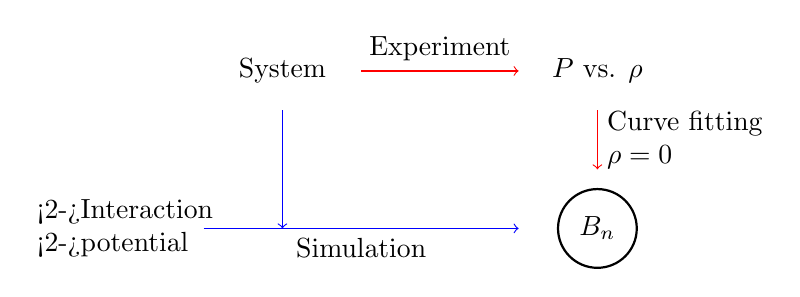
\begin{tikzpicture}
				\node at (-2,3) {System};
				\draw[->,red] (-1,3) -- (1,3);
				\node[above] at (0,3) {Experiment};
				\node at (2,3) {$P$ vs. $\rho$};
				\draw[->,red] (2,2.5) --(2,2.125) node[align=left,right,black]{Curve fitting\\ $\rho = 0$ } -- (2,1.75);
				\node at (2,1) {$B_n$};
				\draw[thick] (2,1) circle [radius=0.5];
				\node[align=left] at (-4,1) {\alert<2->{Interaction}\\ \alert<2->{potential}};
				\draw[->,blue] (-3,1) -- (-1,1) node[below,black] {Simulation} -- (1,1);
				\draw[->,blue] (-2,2.5) -- (-2,1);
				\end{tikzpicture}      
				\end{figure}
				\item \visible<2->{Accuracy of potential models (empirical or \emph{ab initio}) to capture the nature of interactions can be gauged}
			\end{itemize}
		\end{frame}

		\begin{frame}
			\frametitle{Empirical vs. \emph{Ab initio} potential models}
			\begin{itemize} 
				\justifying
				\item Empirical potential models - usually functions fitted to experimental data
				\item Represent the net effect of a variety of phenomenon taking place including 2 body interactions, multi-body interactions, nuclear quantum effects etc.  
				\item As a result, fail to accurately represent interaction potential
				\item Interaction potentials that better represent condensed (high density) phase fail to predict accurate virial coefficients for the gas (low density) phase
			\end{itemize}
		\end{frame}
		
		\begin{frame}
			\frametitle{Example - different empirical models of water}
			\begin{itemize}
				\justifying
				\item Importance of the accuracy of interaction potential\putCitation{Benjamin2007}:
				\begin{figure}
				\centering
				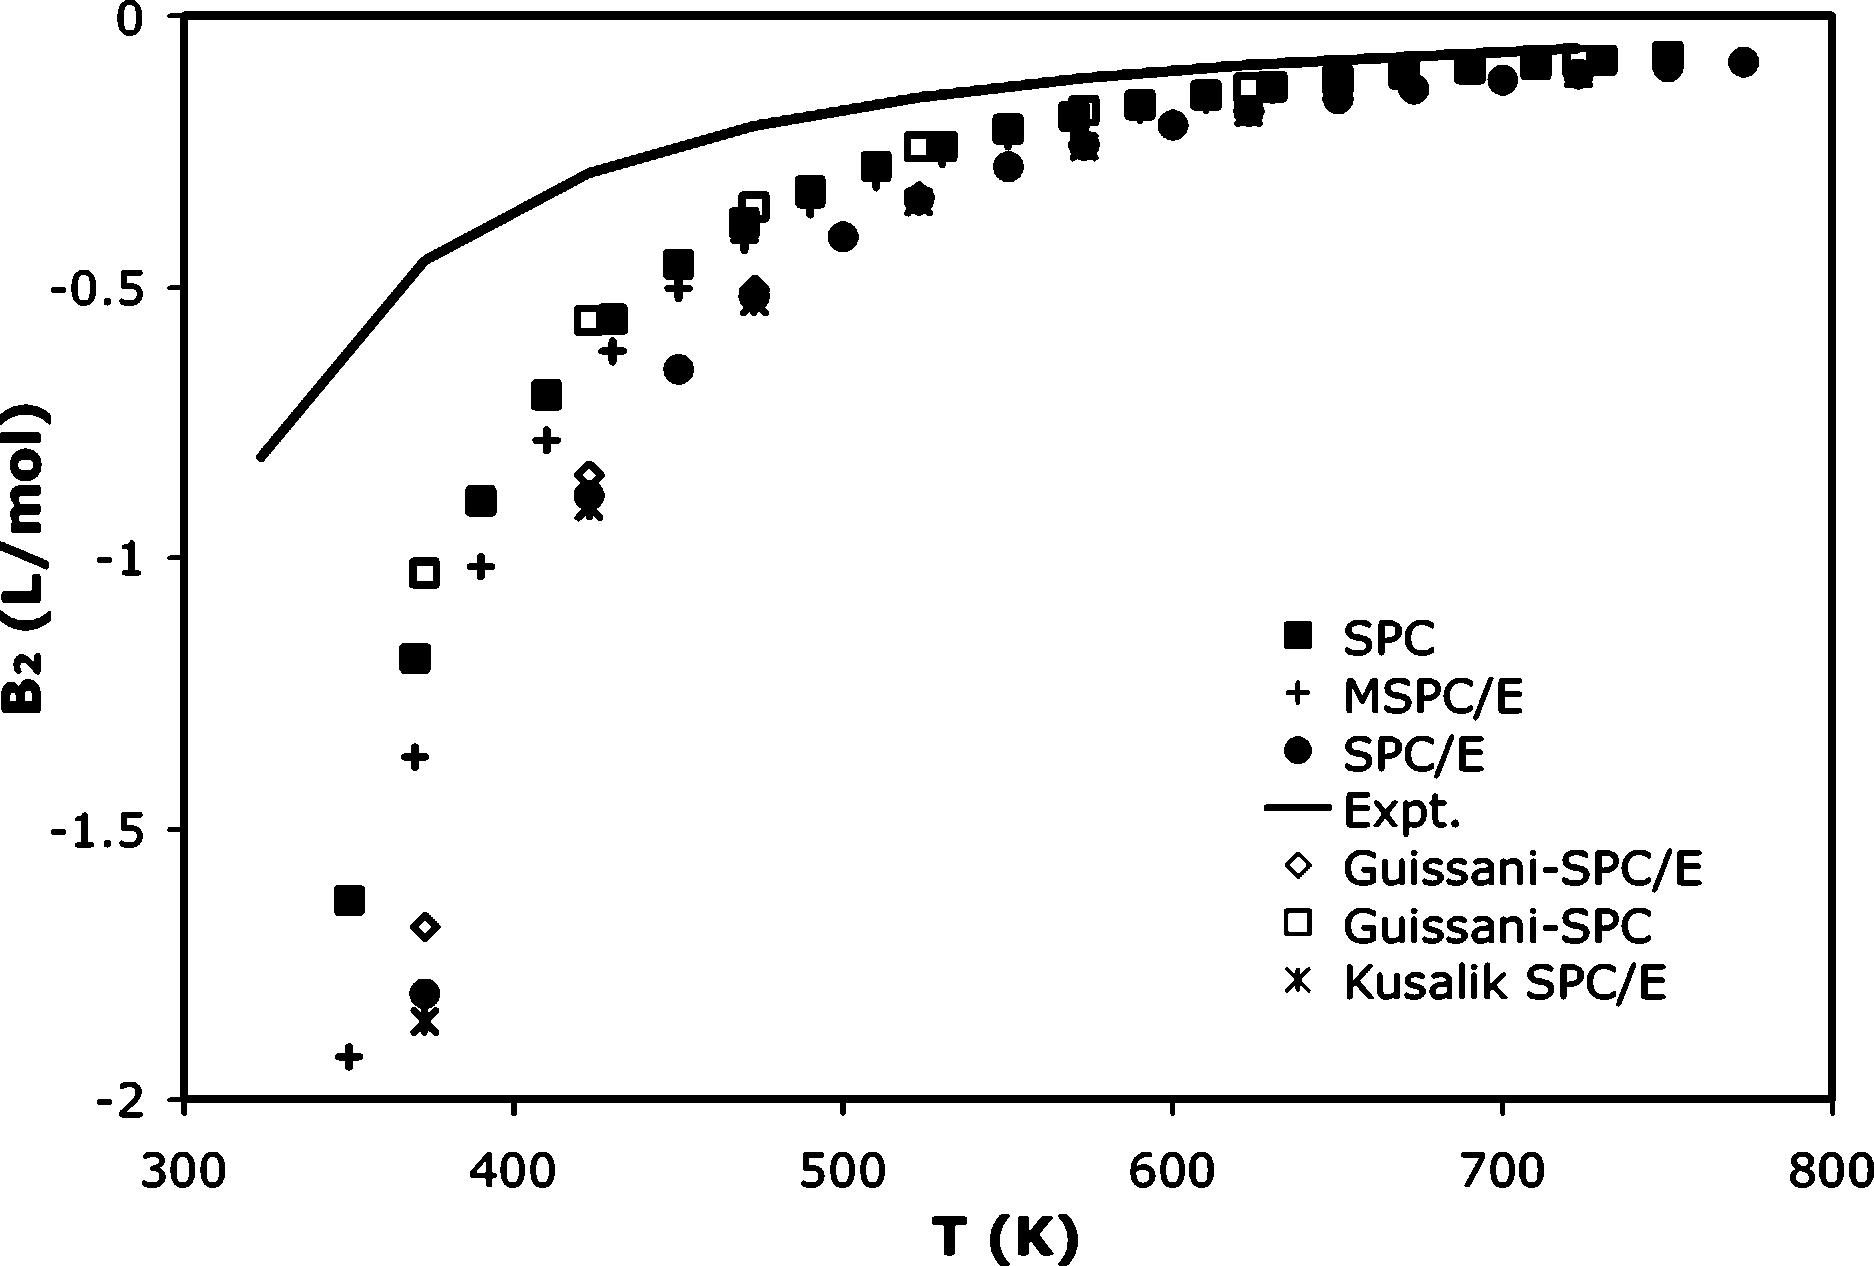
\includegraphics[scale=0.08,keepaspectratio]{ben2a.png}
				\end{figure}
			\end{itemize}
		\end{frame}
	\subsection{Ab initio potentials}
	\section{Objectives}
	\section{Methods}
	\subsection{MSMC}
	\subsection{PIMC}
	\subsection{PIMC with semi-classical beads}
	\section{Results}
	\subsection{Helium-4}
	\subsection{Diatomic molecules}
	\subsection{Water}
	\section{Summary}
	\section*{Ackowledgements}

	\begin{frame}
	\frametitle{\Abinitio{} potential models}
	\begin{itemize} 
		\item We use potentials fitted to \emph{ab initio} data rather than compute it on-the-fly (expensive)
		\item \emph{Ab initio} potential models can help predict properties from first principles
	\end{itemize}
	\end{frame}

	\begin{frame}
	\frametitle{Nuclear quantum effects}
	\begin{itemize}
	\justifying
	\item \emph{Ab initio} calculations account for electronic structure using different levels of theory
	\item Nuclear quantum effects have to be explicitly included. Quantum effects become non-negligible at room temperature for gases like helium and hydrogen\putCitation{Garberoglio2009}
	\item Uncertainty in the positions of atoms at low temperatures (Heisenberg's uncertainty principle)
	\end{itemize}
	\begin{figure}
	\centering
	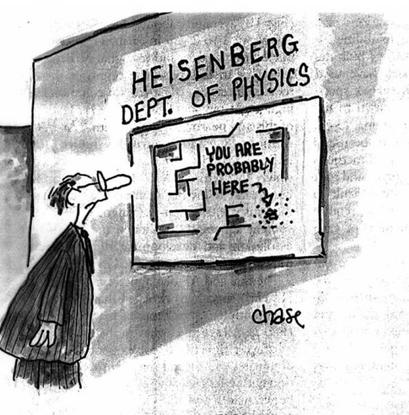
\includegraphics[scale=0.2,keepaspectratio]{uncertaintyPrinciple.jpg}\\
	\tiny{Source: https://www.automationanywhere.com/blog/31-testing-anywhere/317-system-testing-sanity-smoke-and-mirrors}      
	\end{figure}
	
	\end{frame}

	\begin{frame}
	\frametitle{Objectives}
	\begin{itemize}
	\justifying
	\item Use VEOS as a means of testing accuracy of latest \emph{ab initio} potential models\putCitation{Szalewicz2009,Bartolomei2010}
	\item Compute virial coefficients using the most accurate \emph{ab initio} potentials
	\item Understand and develop sampling algorithms to handle rigid and flexible potential models        
	\item Apply PIMC to include nuclear quantum effects in simpler systems e.g. monatomics, diatomics
	\item Ultimate goal: to compute fully quantum virial coefficients for water
	\end{itemize}
	\end{frame}

	\begin{frame}
	\frametitle{Non PIMC approaches to handle nuclear quantum effects}
	\begin{itemize}
	\justifying
	\item Adding a first order quantum correction to classical calculation
	\item Using a more diffusive potential like the Quadratic Feynman-Hibbs\putCitation{Shaul2012}
	\begin{figure}
	\centering
	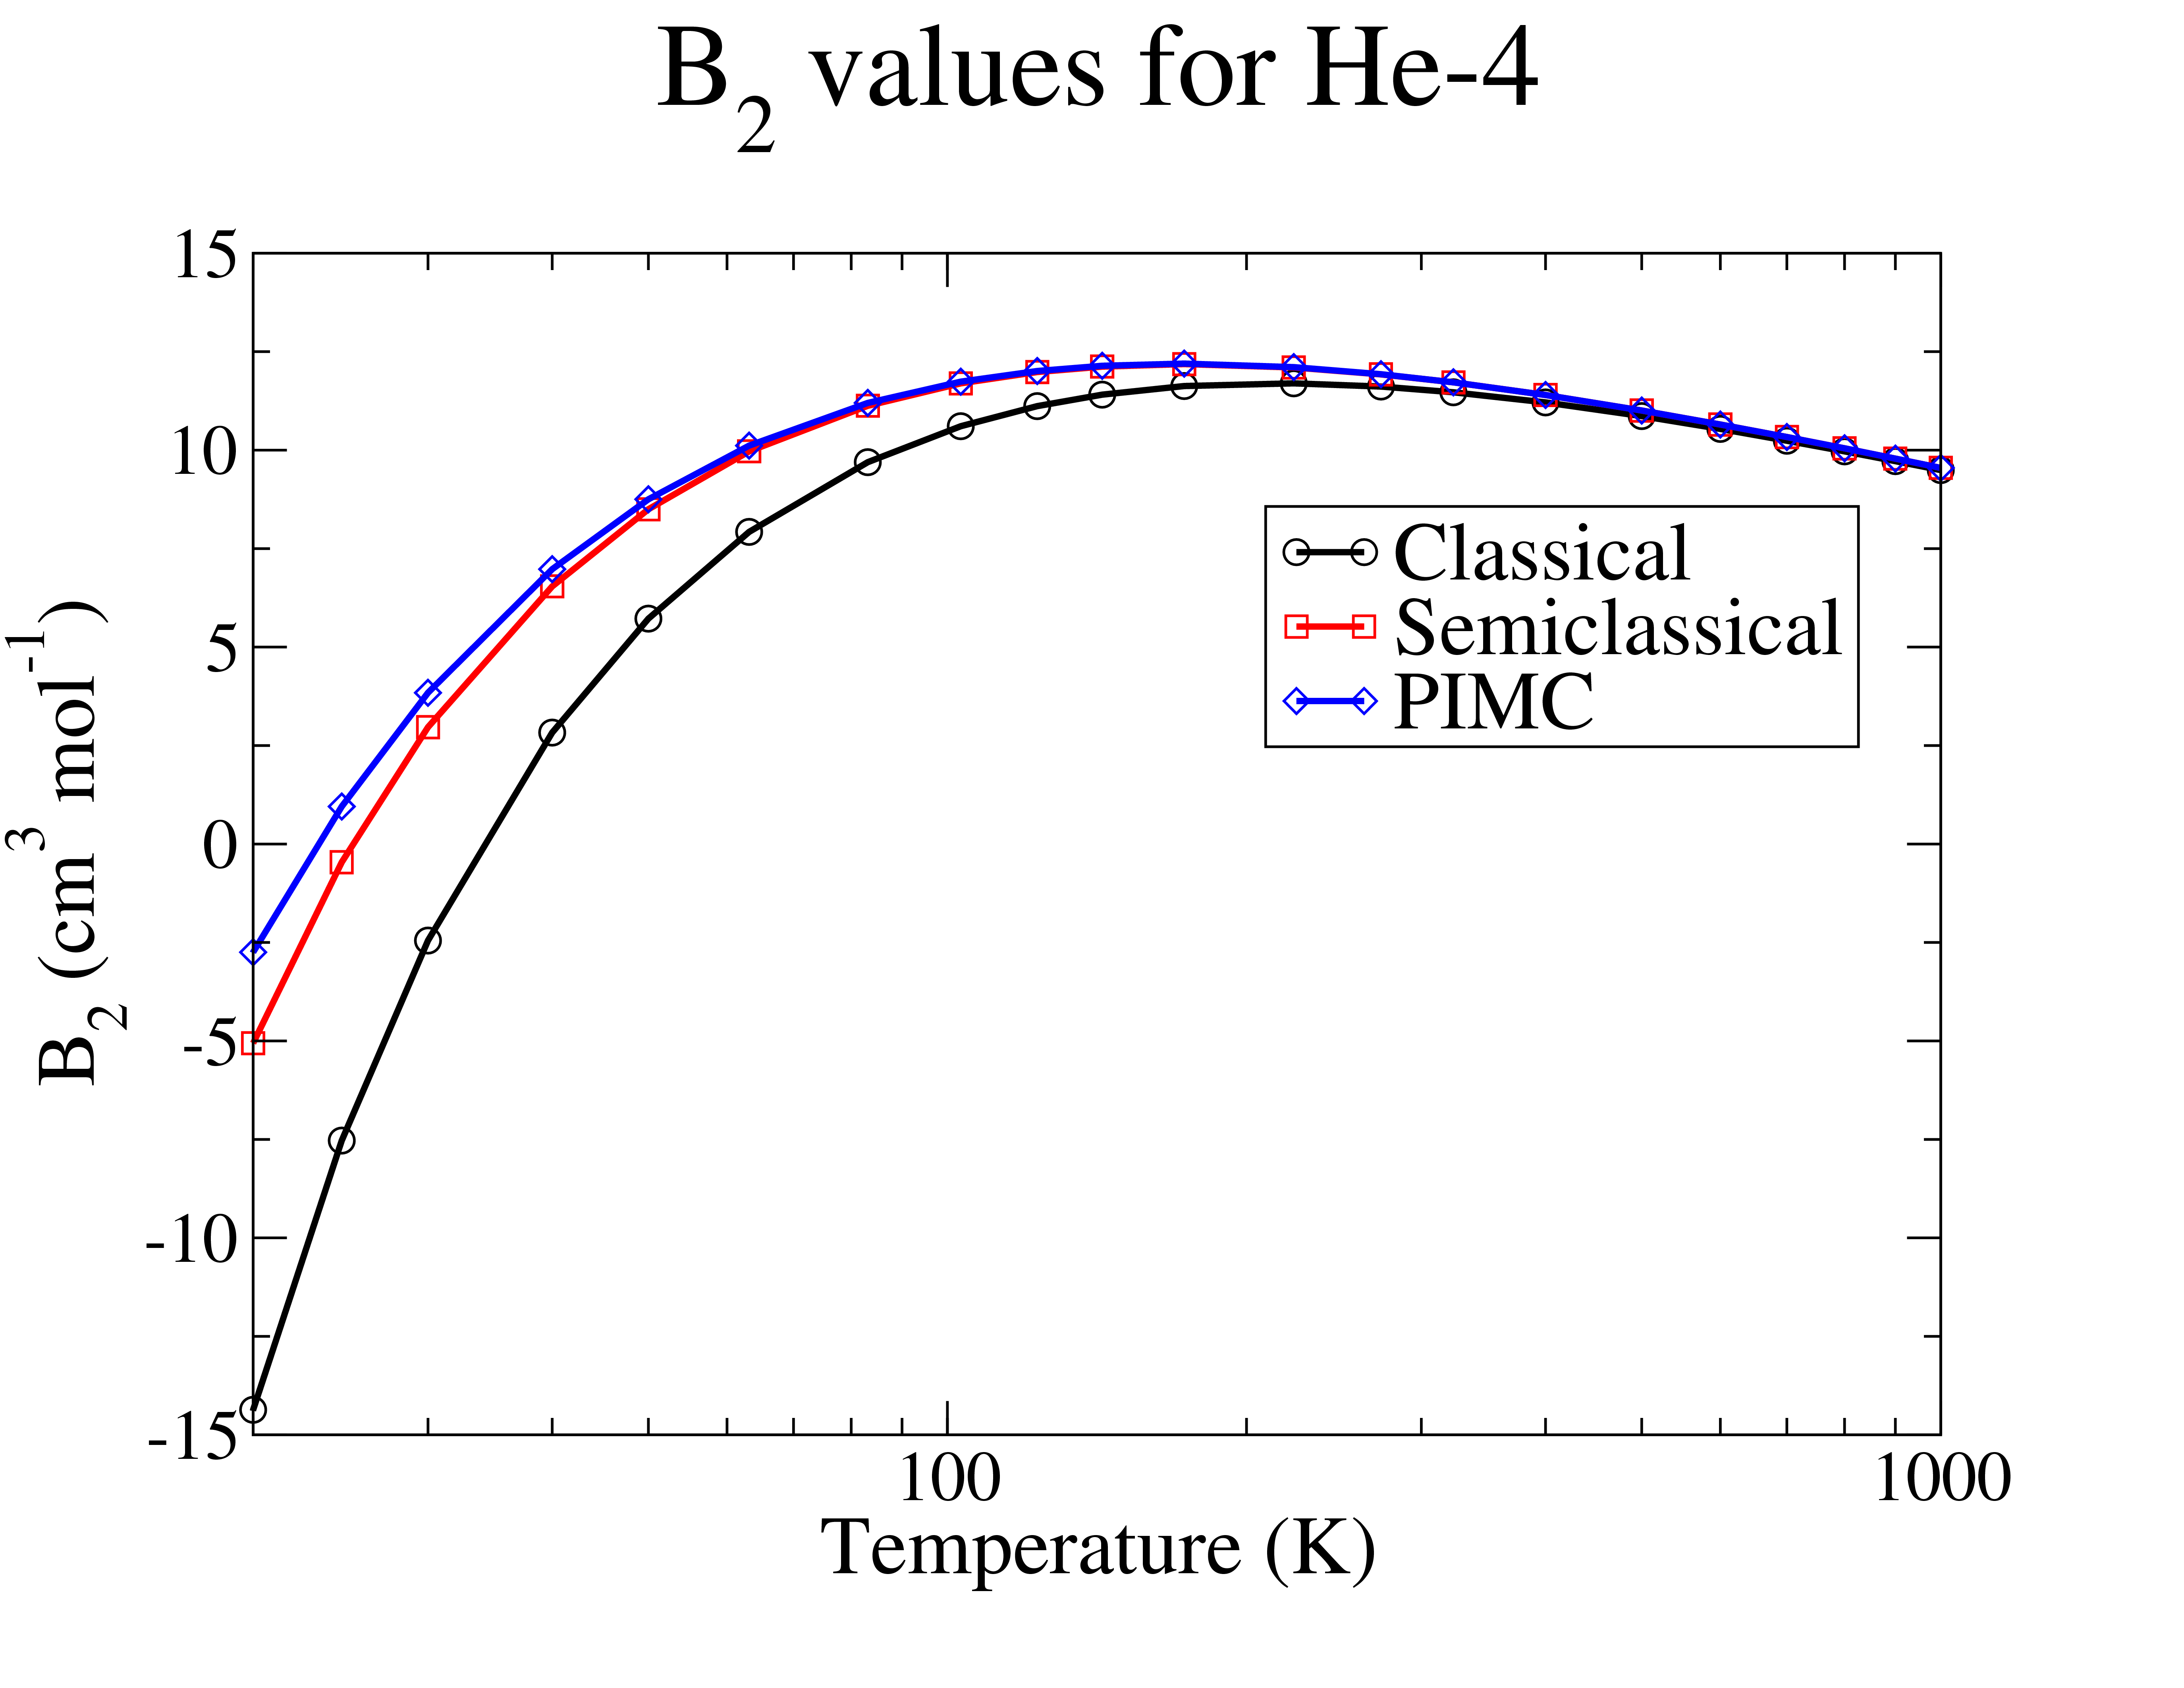
\includegraphics[scale=0.03,keepaspectratio]{B2-Kate.png}
	\end{figure}
	\item At very low temperatures, we still need to use PIMC method to account for complete quantum behavior
	\end{itemize}
	\end{frame}

	\begin{frame}
	\frametitle{PIMC - monatomic molecule e.g. He}
	\begin{itemize}
	\justifying
	\item PIMC - provides a route to incorporate nuclear quantum effects
	\item Kinetic energy effects of the molecule lead to harmonic spring-like interactions between adjacent ``beads"
	\begin{figure}          
	\centering
	\def\svgscale{0.3}
	\input{monatomicPIMC.pdf_tex}
	\end{figure}
	\item Interaction energy is computed as: $U_{int} = \displaystyle\sum\limits_{i=1}^P \frac{U_i}{P}$
	\begin{figure}
	\centering
	\def\svgscale{0.3}
	\input{interactionEnergyMonatomic.pdf_tex}
	\end{figure}
	\item To form a closed ring of springs, the position of each bead needs to be chosen based on a Gaussian distribution. Hence, implementing PIMC is trivial for the monatomic case
	\end{itemize}
	\end{frame}
	
	\begin{frame}
	\frametitle{PIMC results for Helium-4\putCitation{Shaul2012}}
	\begin{figure}
	\centering
	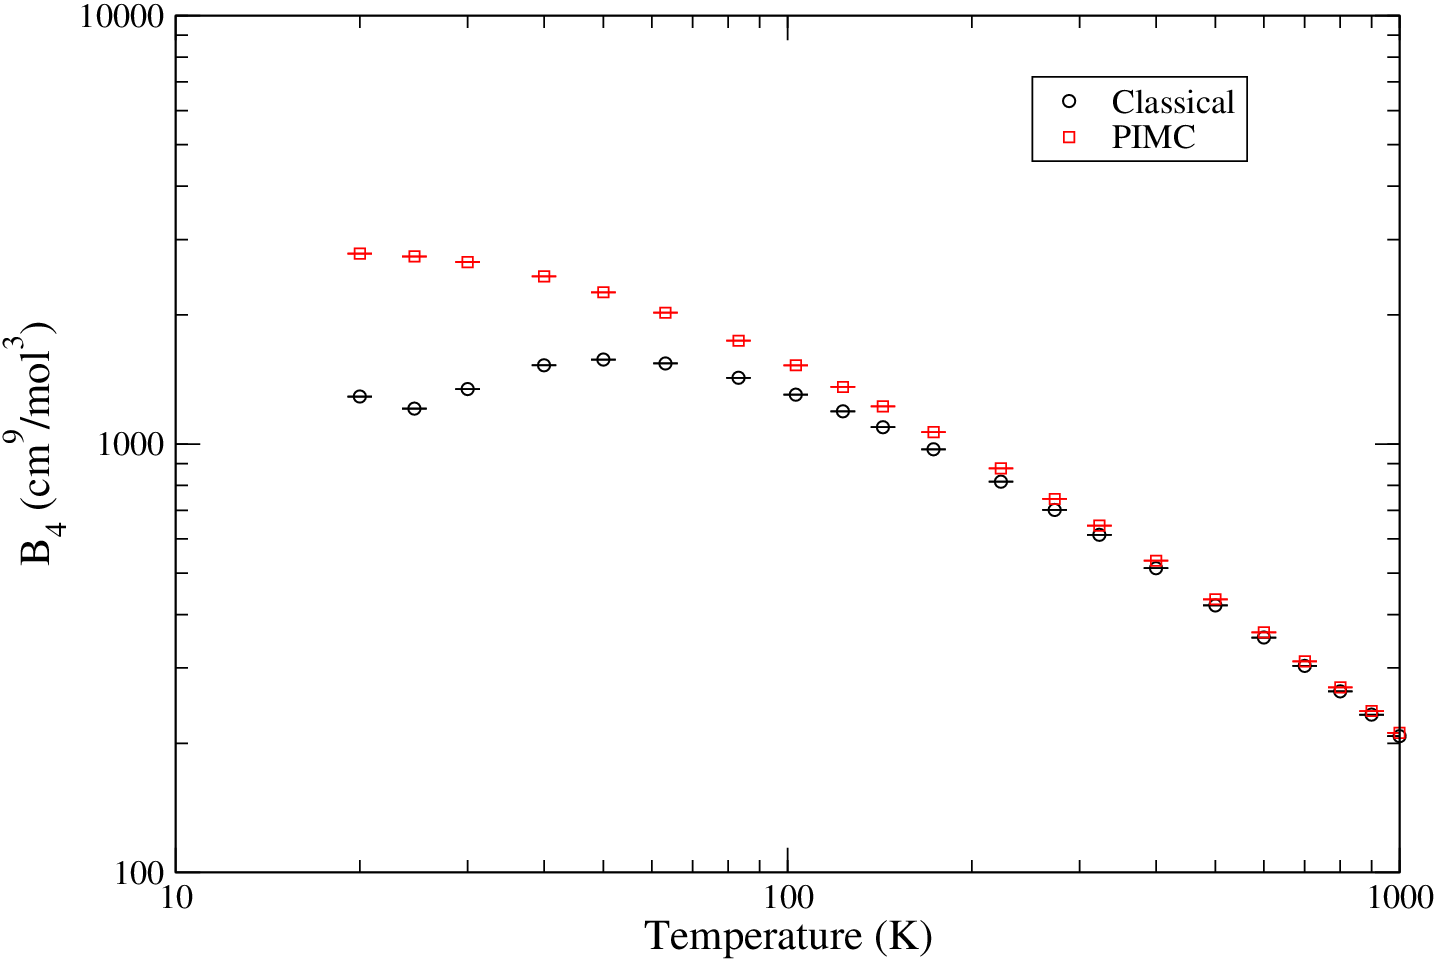
\includegraphics[scale=0.2,keepaspectratio]{B4-Kate.png}
	\end{figure}
	\end{frame}

	\begin{frame}
	\frametitle{PIMC - rigid diatomic molecule}
	\begin{itemize}
	\item Probability distribution for choosing an orientation is not Gaussian
	\item Probability of choosing adjacent orientation is exact and analytic but we can't form a ring if we choose from that distribution
	\begin{figure}
	\centering
	\def\svgscale{0.2}
	\input{orientationRD.pdf_tex}
	\end{figure}
	\item Entire difficulty lies in coming up with a probability distribution for non-adjacent monomer orientations which results in closed ring configurations
	\begin{figure}
	\centering
	\def\svgscale{0.3}
	\input{diatomicPIMC.pdf_tex}
	\end{figure}
	\end{itemize}
	\end{frame}
	
	\begin{frame}
	%slide 8
	\frametitle{A new orientational sampling algorithm}
	\begin{itemize}%[<+->]
	\item What if we don't model using the quantum rigid rotor approximation? 
	\item The only factor that affects the probability of any configuration is the \alert{harmonic spring-like interaction} between adjacent beads 
	\item $U_h = \displaystyle\sum\limits_{\# rings} \displaystyle\sum\limits_i k_h |\textbf{x}_i - \textbf{x}_{i-1}|^2 ,\text{with} \: k_h = \frac{\pi P}{\Lambda^2}$ where $\Lambda = \frac{h}{\sqrt{2 \pi m k_B T}}$ \: and $\textbf{x}_i$ denotes position of the bead $i$
	\item The actual probability of any configuration is given by $P_{act} = exp(-U_h) $
	\end{itemize}
	\end{frame}

	\begin{frame}
	\frametitle{Growing the ring}
	\begin{itemize}%[<+->]
	\item Tight coupling between adjacent beads makes it difficult to sample orientations that are different, thus lowering the sampling efficiency
	\item We always \alert{grow the complete ring each time} and  we do so \alert{non-sequentially}
	\end{itemize}
	\end{frame}

	\begin{frame}
	\frametitle{Non-sequential algorithm}
	%slide 9
	\begin{itemize}%[<+->]
	\begin{columns}[c]
	\column{6cm}
	\item Image 0 and image P are one and the same. The choice of orientation of image 0 is arbitrary
	\item Each image(child) has a set of two(parent) orientations which affect where it is placed
	\item For each pass, we need a probability distribution of the child image that depends on the orientations of both the parent images

	\column{3.4cm}
	\vspace{0cm}
	\begin{overlayarea}{3.5cm}{3.5cm}
	\begin{figure}[H]
	\only<1>{
	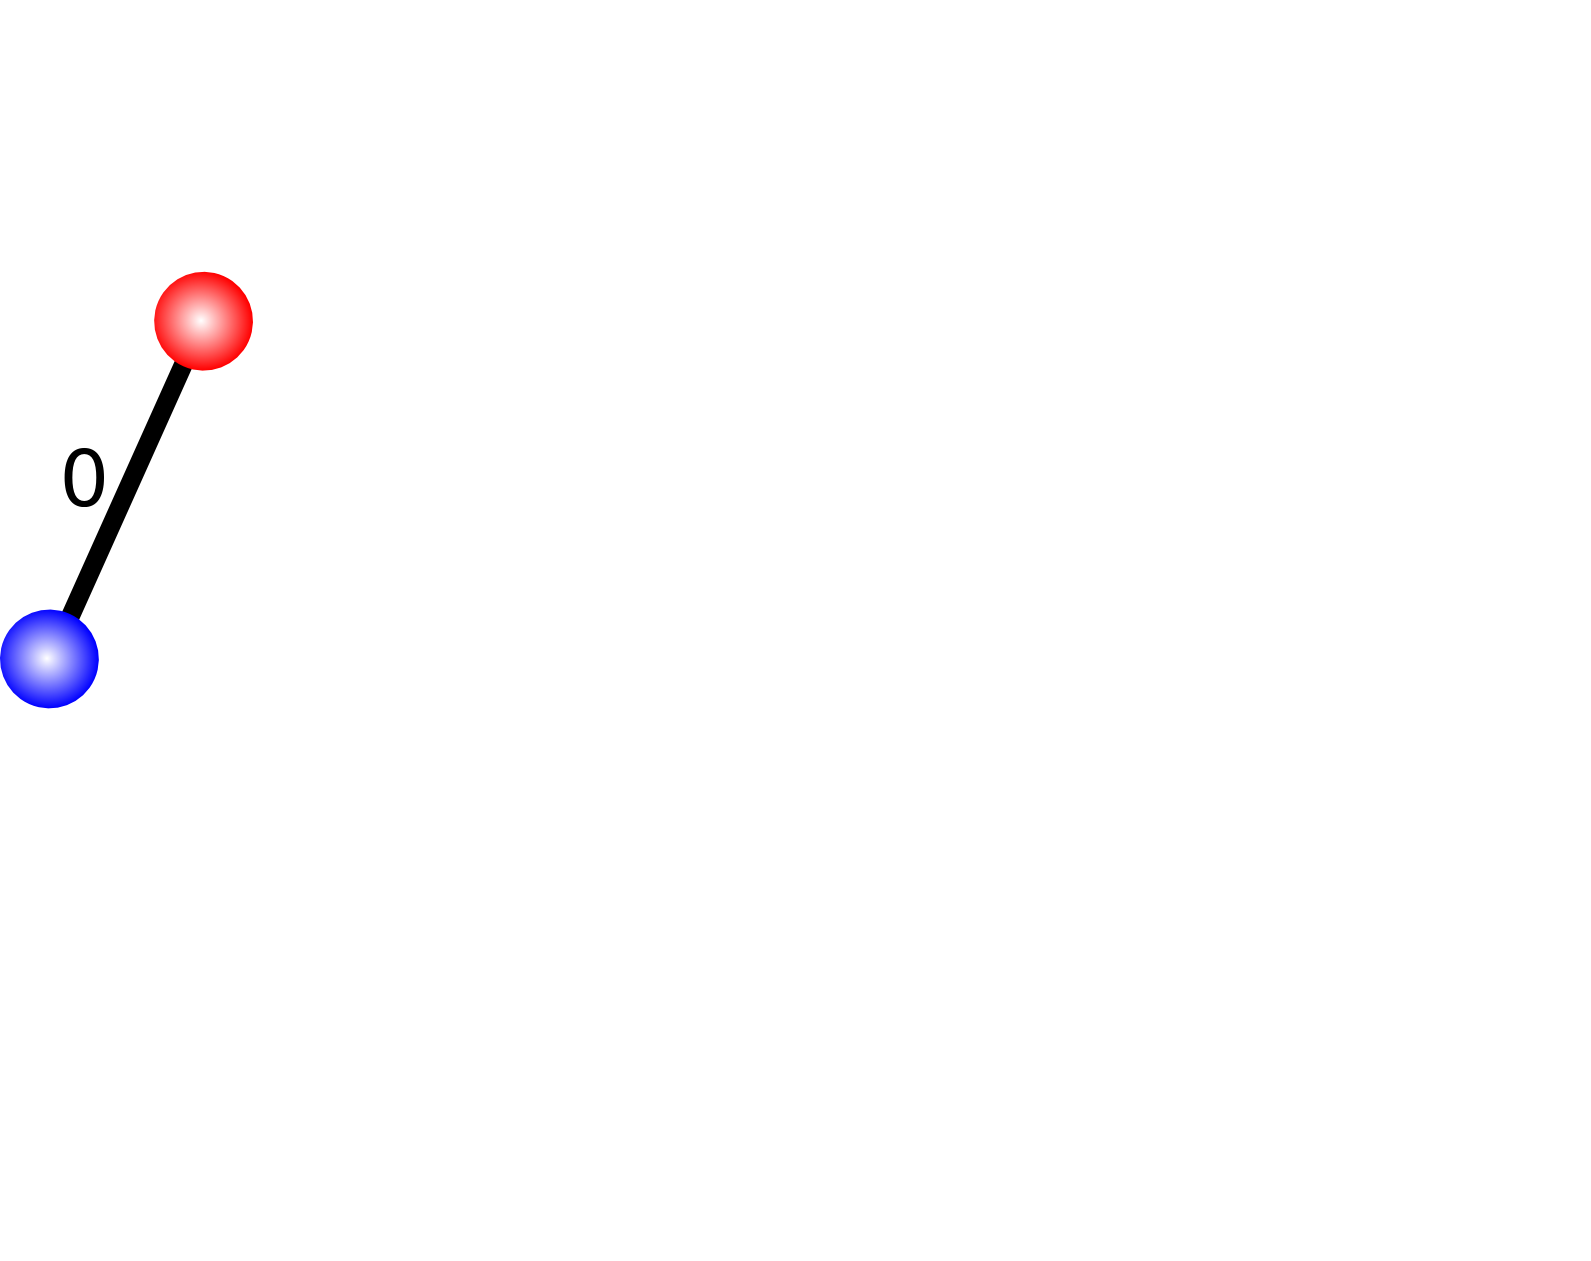
\includegraphics[width=3.5cm,height=3.5cm,keepaspectratio]{ns0.png}
	\caption{Example for P = 8}
	}
	\only<2>{
	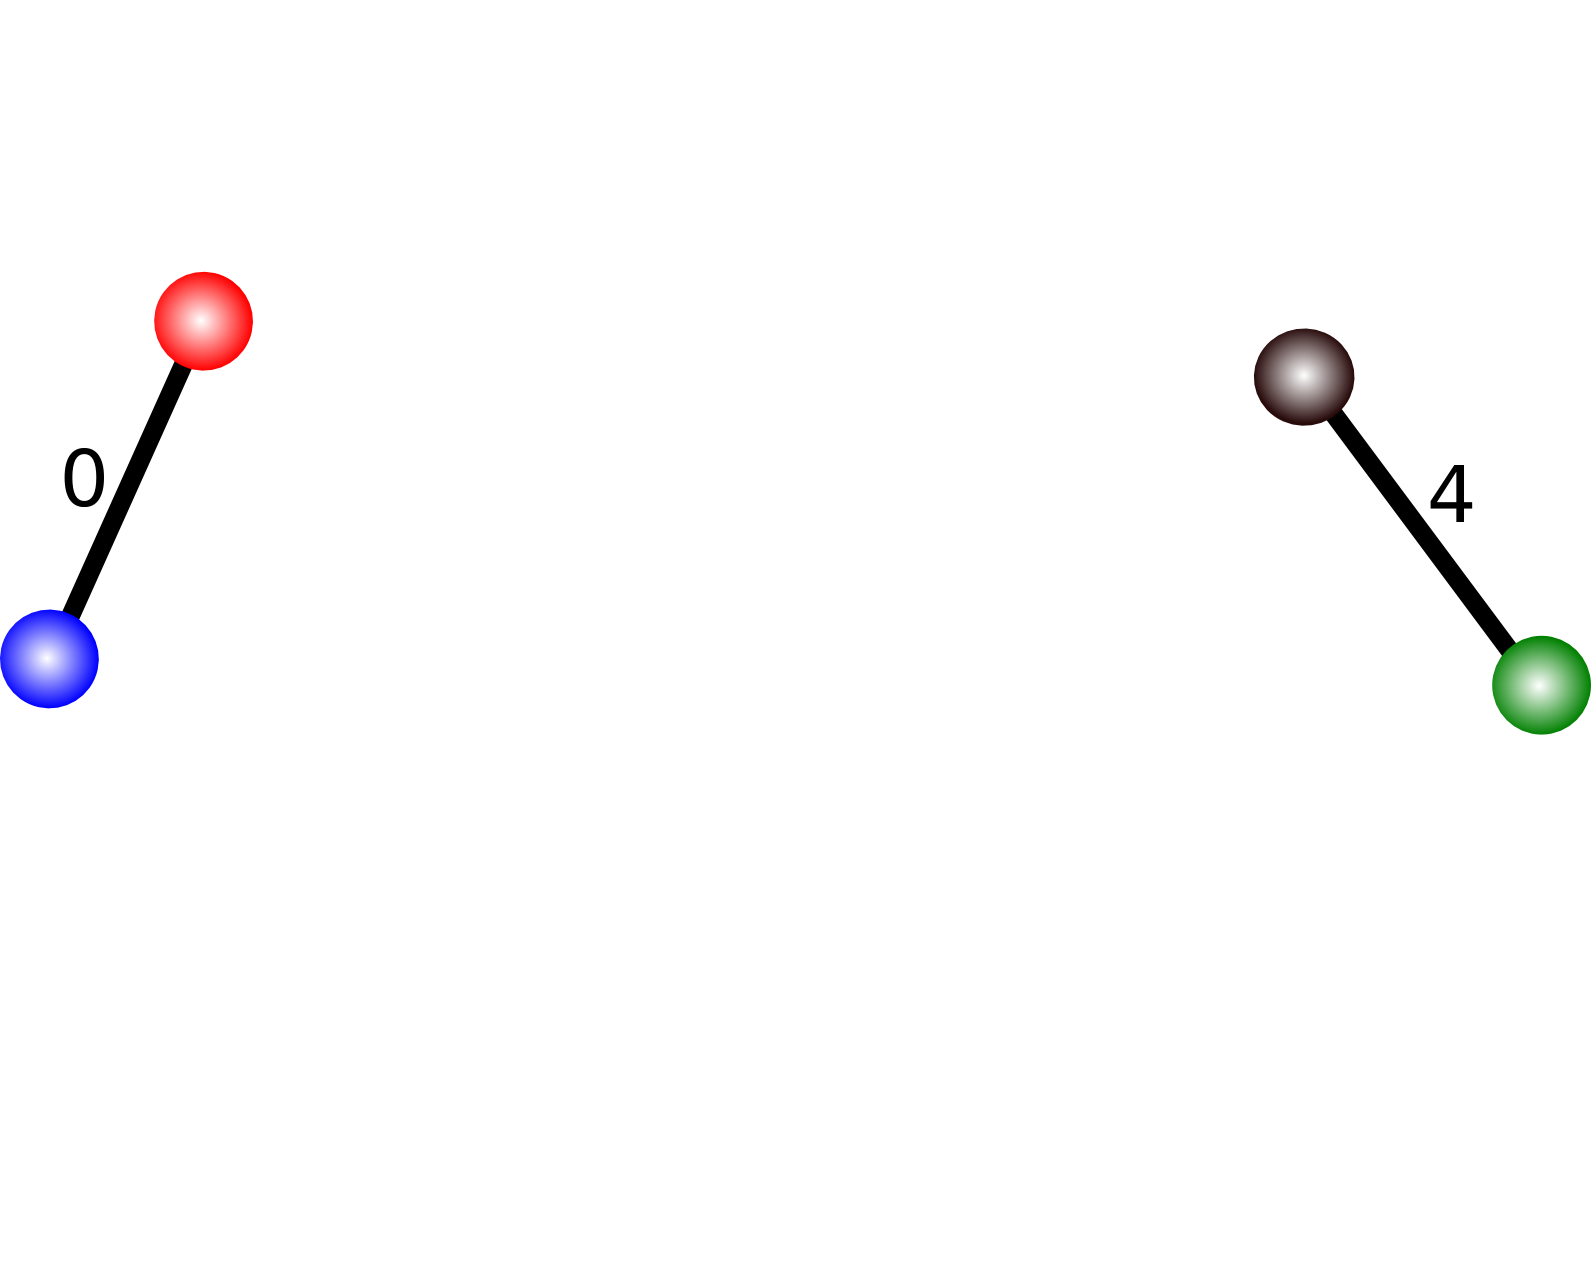
\includegraphics[width=3.5cm,height=3.5cm,keepaspectratio]{ns04.png}
	\caption{Example for P = 8}
	}
	\only<3>{
	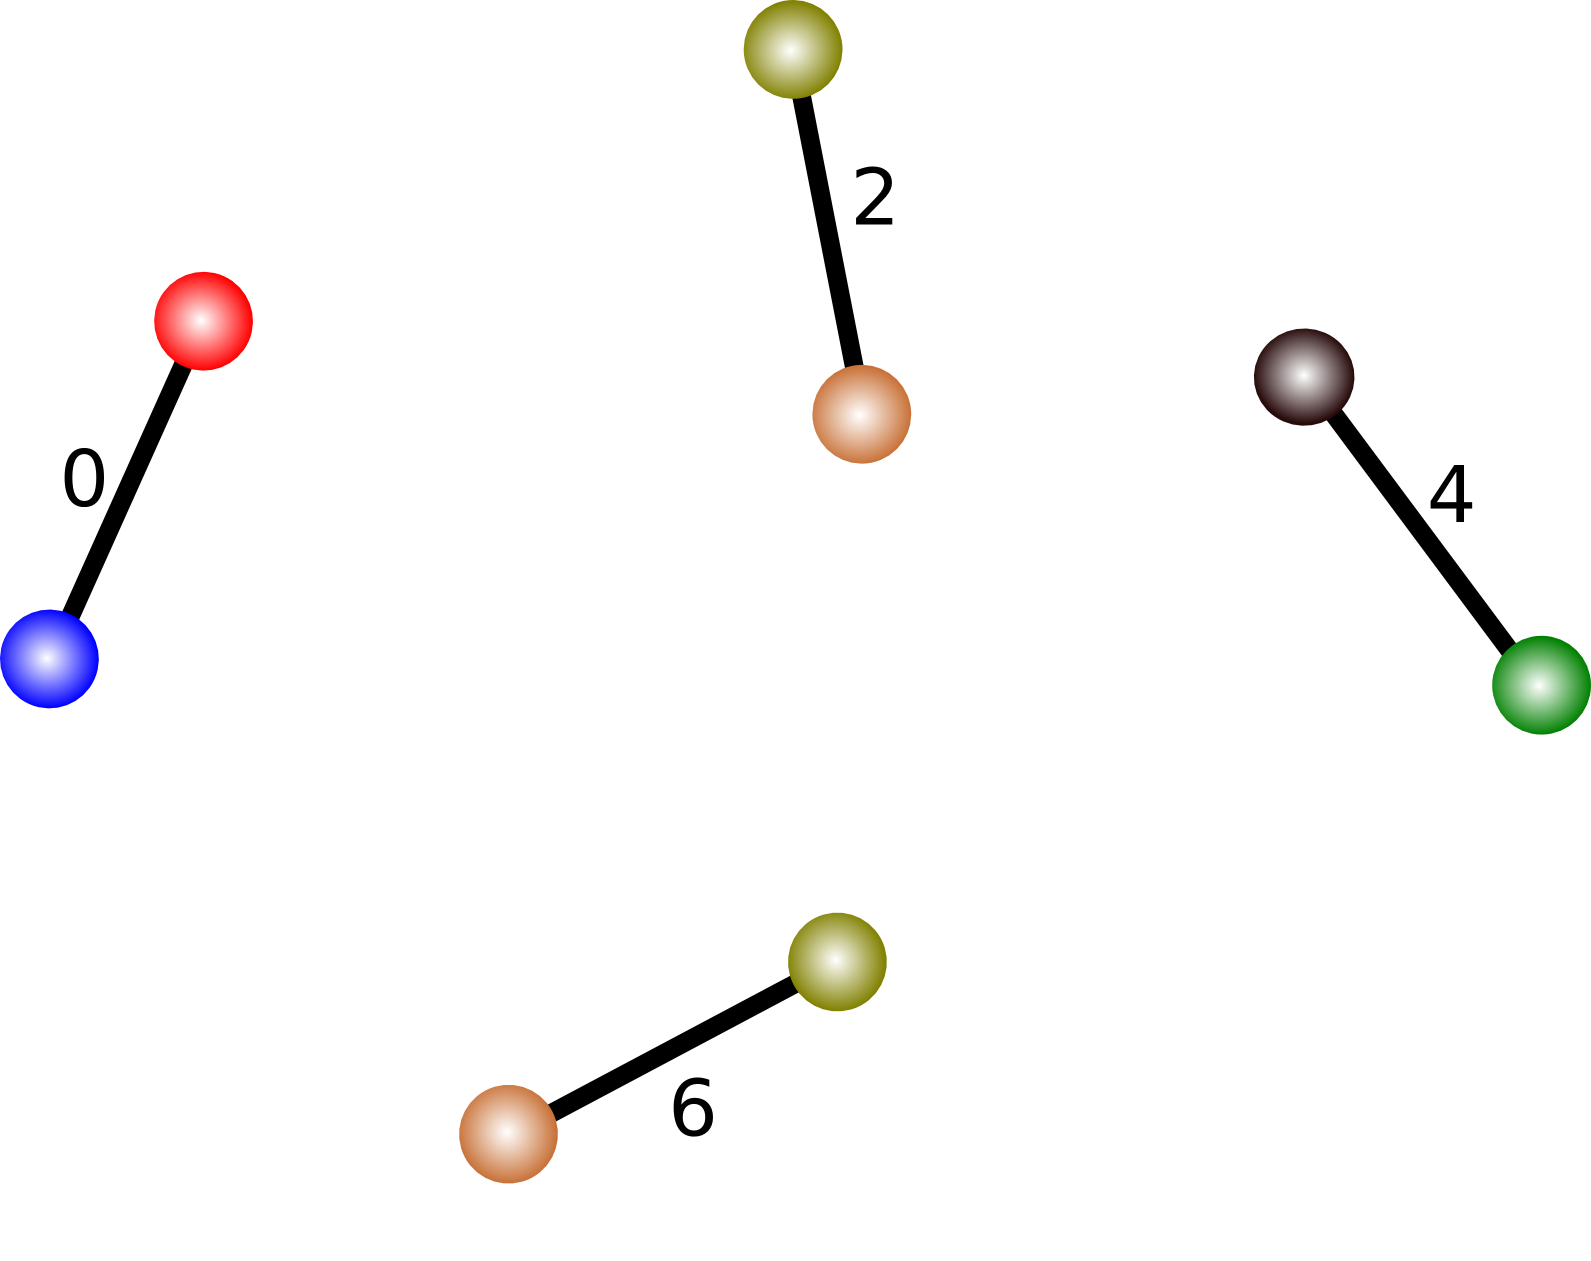
\includegraphics[width=3.5cm,height=3.5cm,keepaspectratio]{ns0426.png}
	\caption{Example for P = 8}
	}
	\only<4>{
	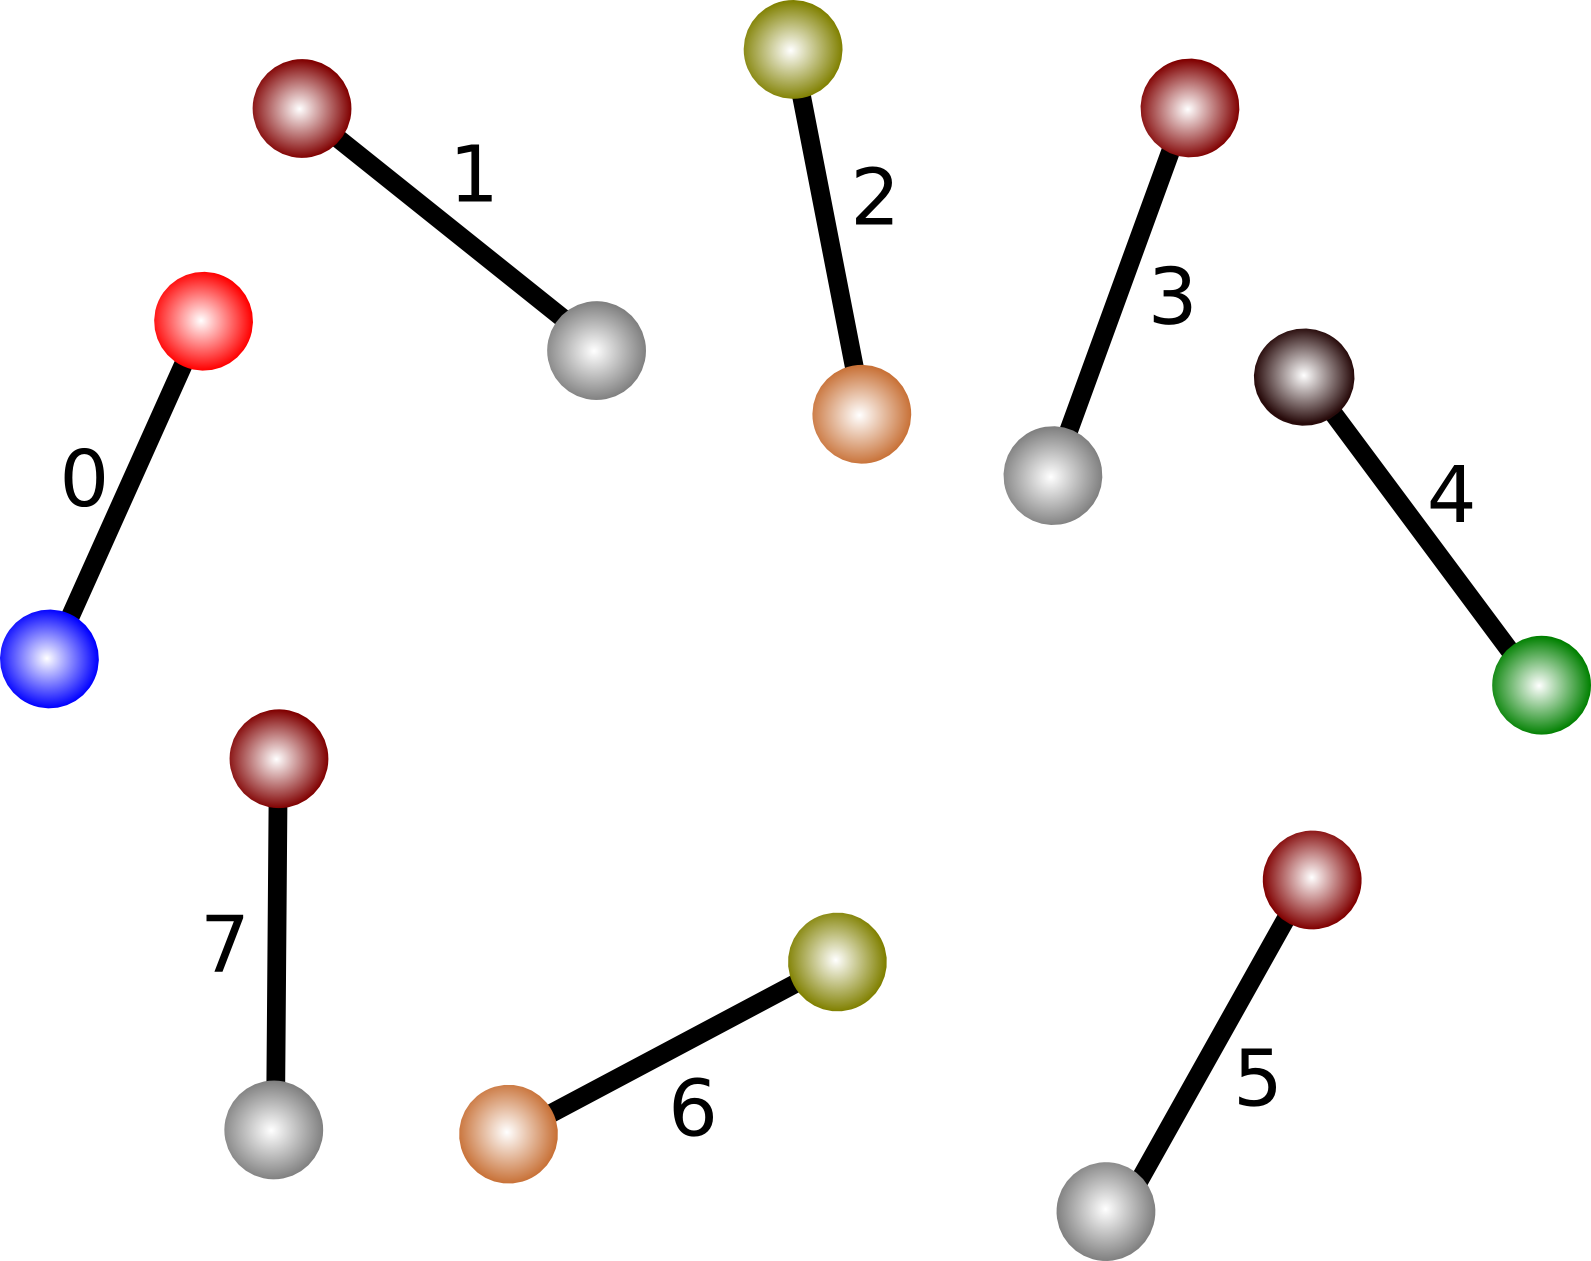
\includegraphics[width=3.5cm,height=3.5cm,keepaspectratio]{nsall.png}
	\caption{Example for P = 8}
	}
	\end{figure}
	\end{overlayarea}
	\end{columns}
	\end{itemize}
	\end{frame}

	\begin{frame}
	%slide 10
	\frametitle{Adjacent image probability $P_{01}$}
	\begin{itemize}%[<+->]
	\begin{columns}[t]
	\column{6cm}
	\item Consider a sphere with diameter $=$ bond length of the molecule i.e. $r = b/2$ 
	\item Let image `0' be oriented along the z-axis and image `1', at angle \:$\phi_1$\: away from it
	\item Distance `x' between beads of adjacent images is given by $x^2 = 2 r^2 ( 1 - cos \phi_1)$
	\column{3.4cm}
	\begin{figure}
	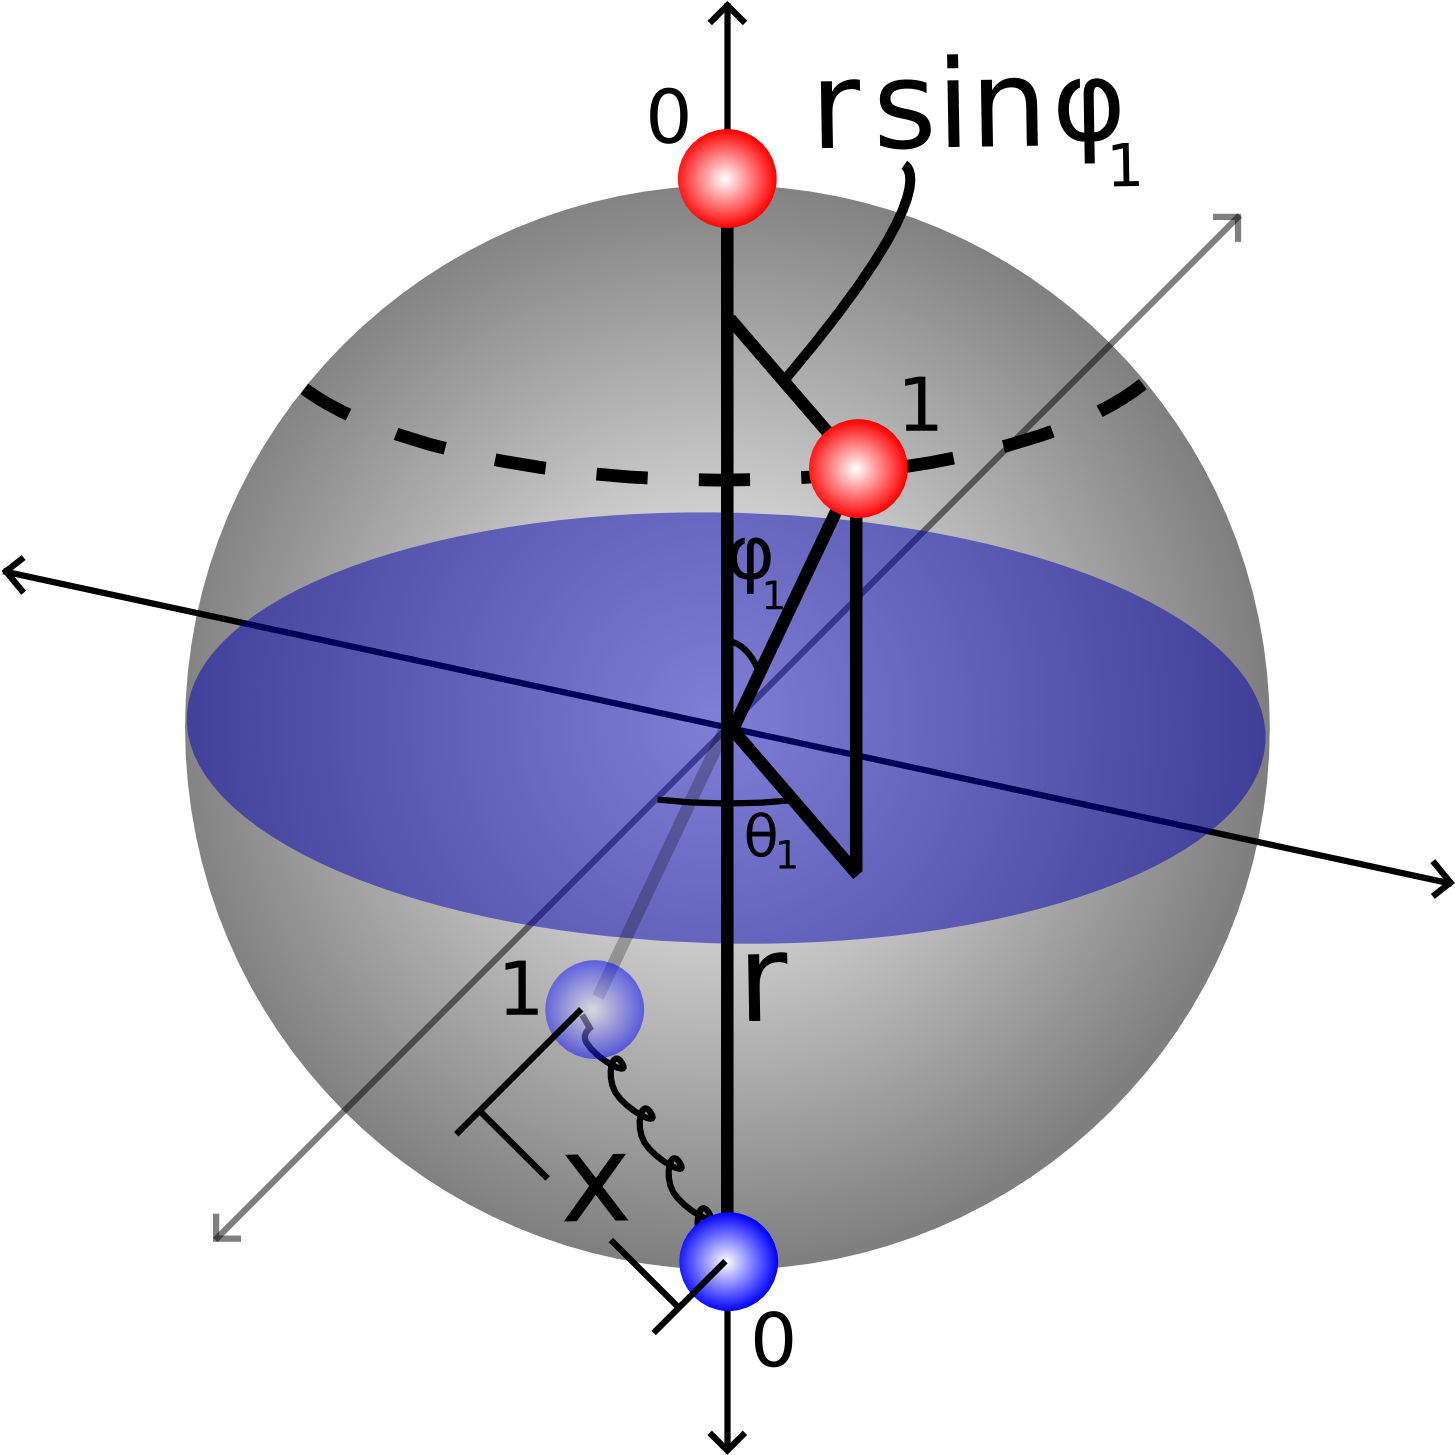
\includegraphics[width=\textwidth,keepaspectratio]{degeneracyNew.png}
	\caption{P = 2 case}
	\end{figure}
	\end{columns}
	\item The harmonic interaction energy is given by, $U_h = 4 k_h r^2 (1 - cos \phi_1)$
	\item $P_{01}$ is given by:
	\begin{align}
	P_{01} (\phi_1) = exp [-4k_h r^2 (1 - cos \phi_1)]
	\end{align}
	\end{itemize}
	\end{frame}

	\begin{frame}
	%slide 11
	\frametitle{Comparison between algorithms\putCitation{Patkowski2008}}
	Normalize these the two functions $P_{01}, \rho$ :
	\begin{align*}
	P_{01} (\phi_1) = &exp [ -4 k_h r^2 (1 - cos \phi_1) ] \\
	\rho(\phi_1) = &\frac{1}{q_{rot}} \displaystyle\sum\limits_{j=0}^{100} \frac{2j+1}{4 \pi} P_j (cos \phi_1) \times exp[- \beta j (j+1)\Upsilon /P]
	\end{align*}       
	\begin{center}
	\begin{figure}
	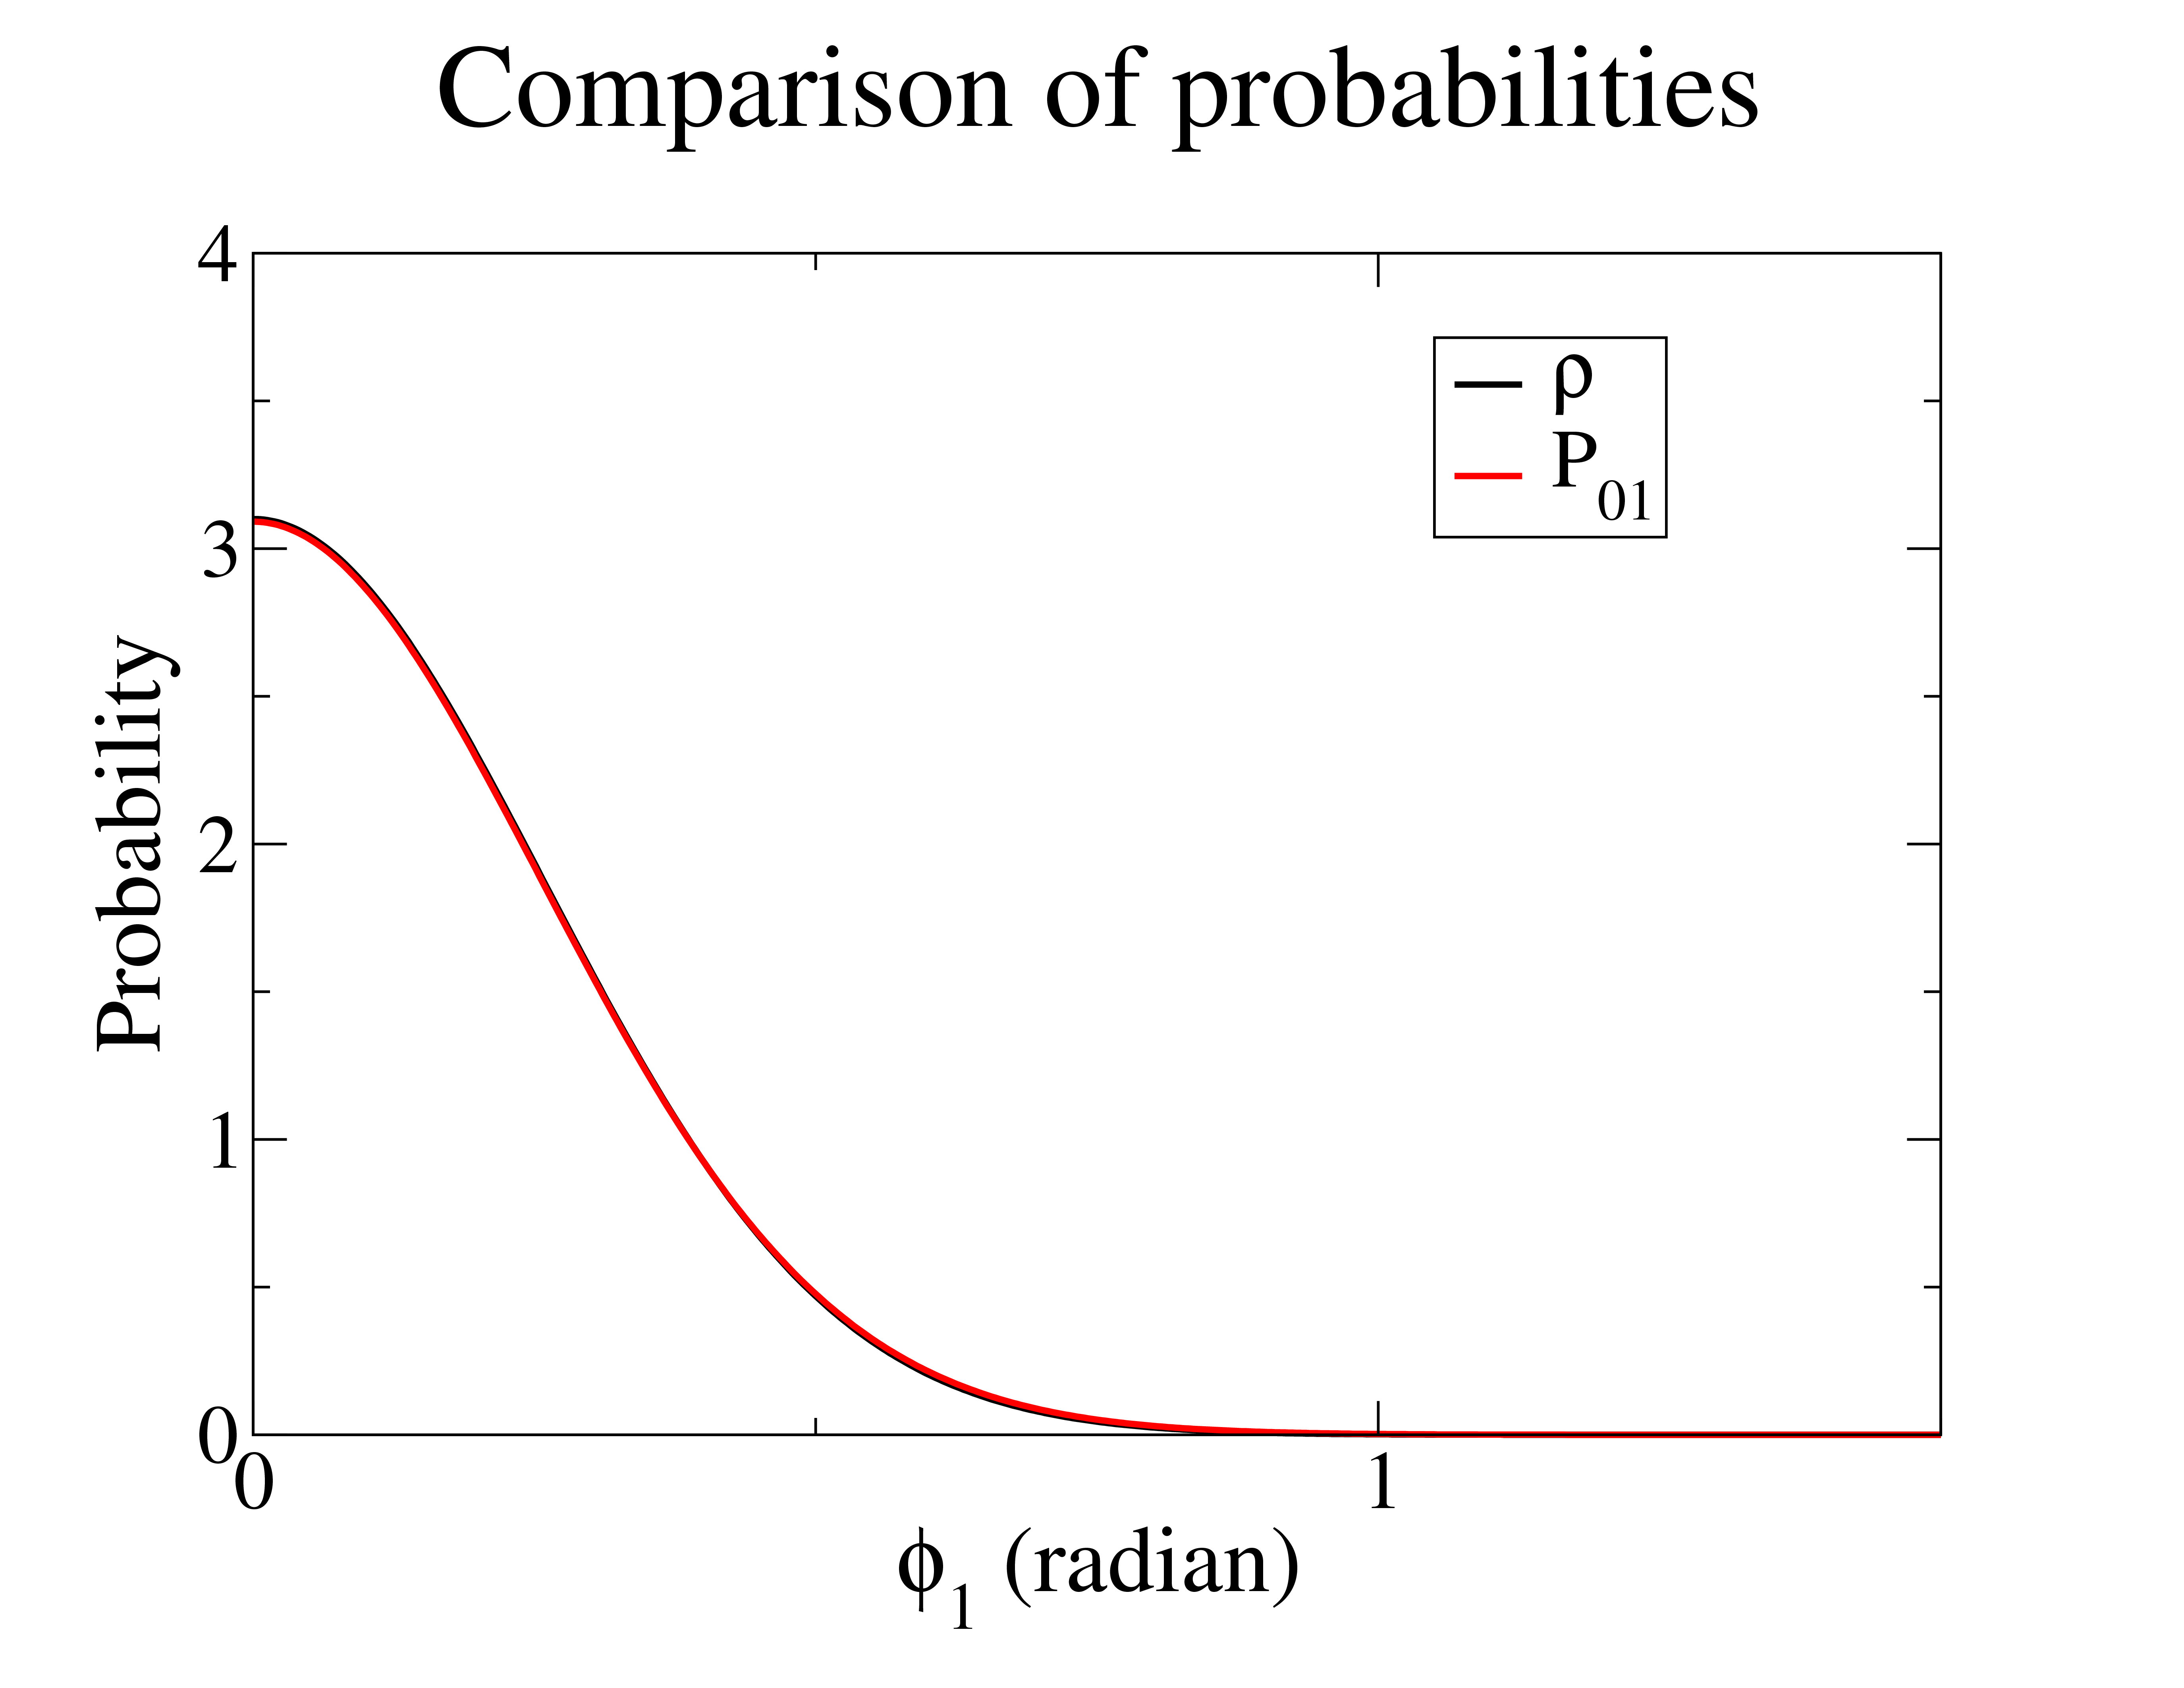
\includegraphics[width=5.5cm,keepaspectratio]{probabilityComparison.png}
	\end{figure}
	\end{center}
	\end{frame}

	\begin{frame}
	%slide 12
	\frametitle{Parent $\to$ child}
	\begin{itemize}%[<+->]
	\item Given two parent images $I_1,I_2$, the harmonically most favorable orientation for the child image is the average of the their orientations
	\item Let $c_n$ denote the average orientation of the two parents for image n and $P_{c_n,I_1 I_2}$ denote the probability distribution centered around $c_n$ 
	\item For the case of $n = 1, P_{c_1,02}$ can be computed analytically
	\begin{center}
	\begin{figure}
	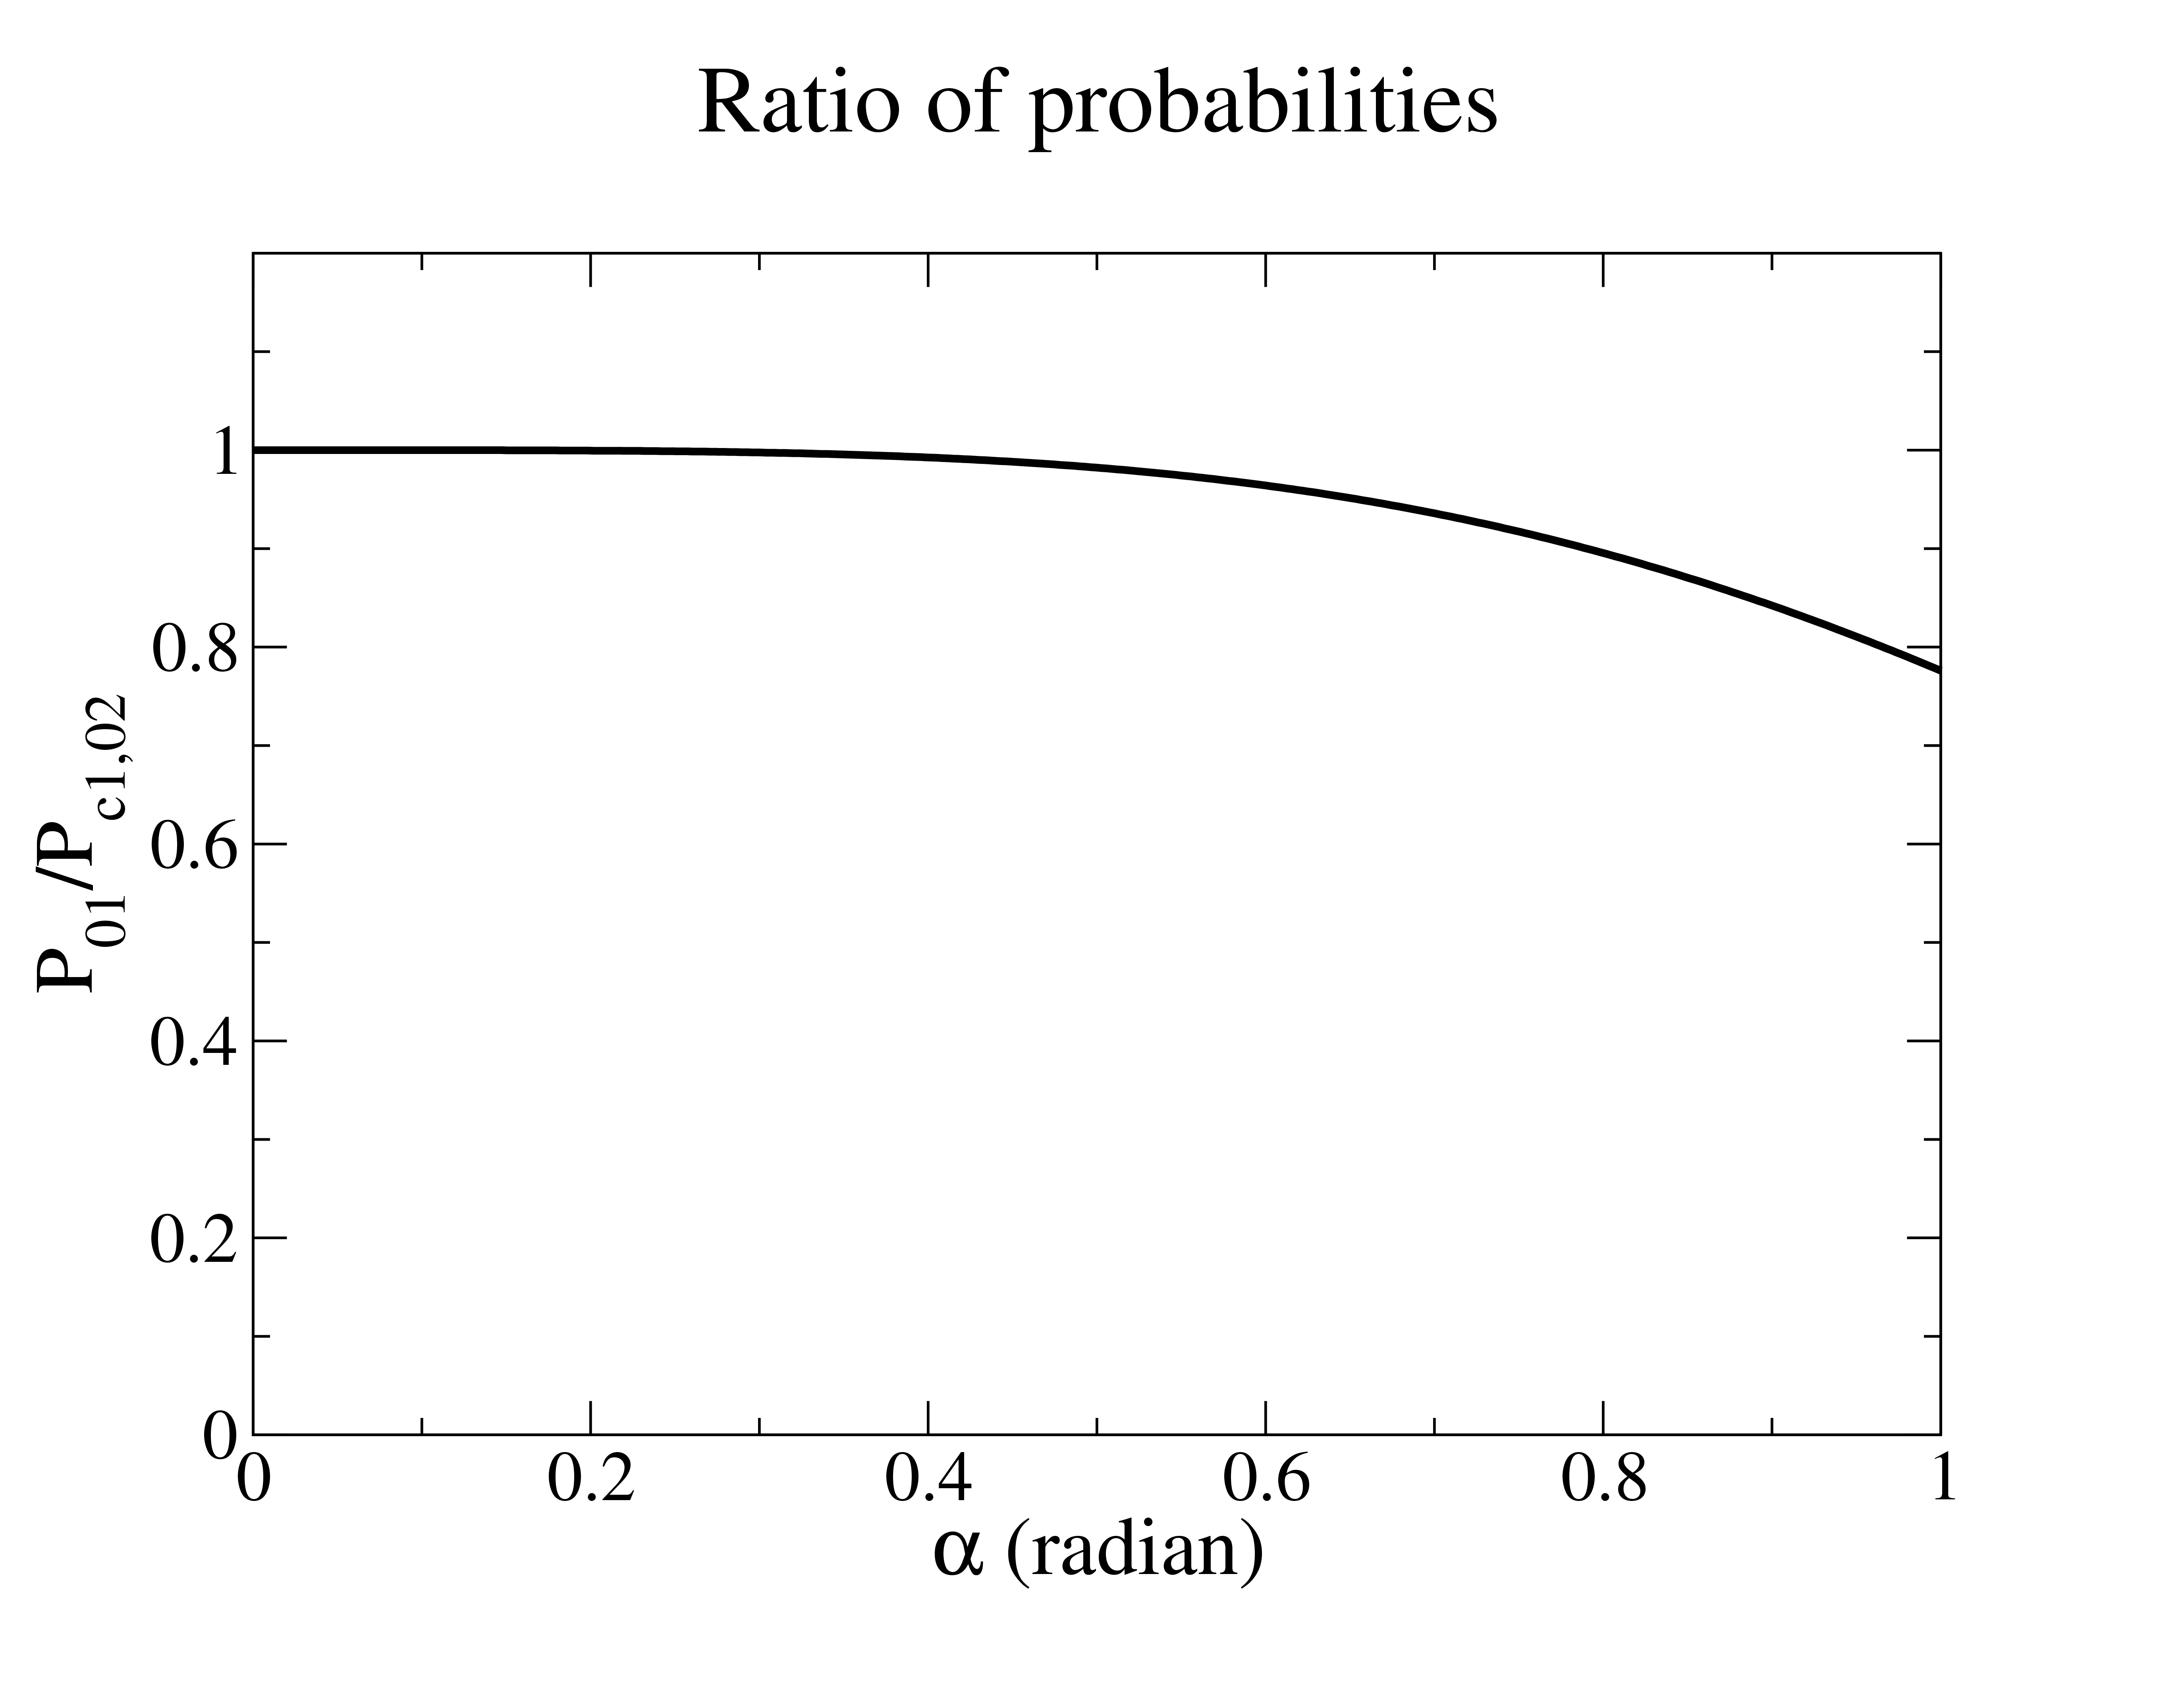
\includegraphics[width=6cm,keepaspectratio]{yratio.png}
	\end{figure}
	\end{center}
	\end{itemize}
	\end{frame}

	\begin{frame}
	%slide 13
	\frametitle{Parent $\to$ child}
	\begin{itemize}%[<+->]
	\item We performed MC simulations and collected histograms of angles $\phi_2 , \phi_4, \phi_8 \ldots$ and observed that:
	\begin{align*}
	&P_{c_n,I_1 I_2} (\phi_n) \approx P_{01} (k_n^{eff},\phi_n) \\
	&k_n^{eff} \propto k_h cos(\psi_n/2)
	\end{align*}
	where $\psi_n$ is the angle between the orientations of $I_1 , I_2$
	\item For the first pass alone, set $I_1 = 0, I_2 = 0$ and subsequent passes will have different sets of parents
	\item Cummulative distribution function:
	\begin{align}
	C(\alpha) = \frac{e^{2k_n^{eff}} - e^{k_n^{eff} (1 + cos \alpha)}}{e^{2k_n^{eff}} - 1}
	\end{align}
	\item Simple and \alert{computationally inexpensive}
	\end{itemize}
	\end{frame}

	\begin{frame}
	%slide 14
	\frametitle{Generating configurations}
	\begin{itemize}
	\item Difficult to generate configurations based on the actual distribution that we desire
	\item Instead we can generate angles from an approximate distribution $C(\alpha)$ much easily
	\item Need to account for it by computing the ratio of the actual and generating probabilities of a configuration
	\item Our acceptance probability is given as: $P_{acc} = \frac{P_{act}^{new}/P_{act}^{old}}{P_{gen}^{new}/P_{gen}^{old}}$
	\item Accept/reject based on $P_{acc}$ and we can sample the (desired) actual distribution more \alert{accurately and efficiently}
	\end{itemize}
	\end{frame}
	
	\begin{frame}
	\frametitle{Bond length \putCitation{Garberoglio2014}- $r_0$}
	\begin{figure}
	\centering
	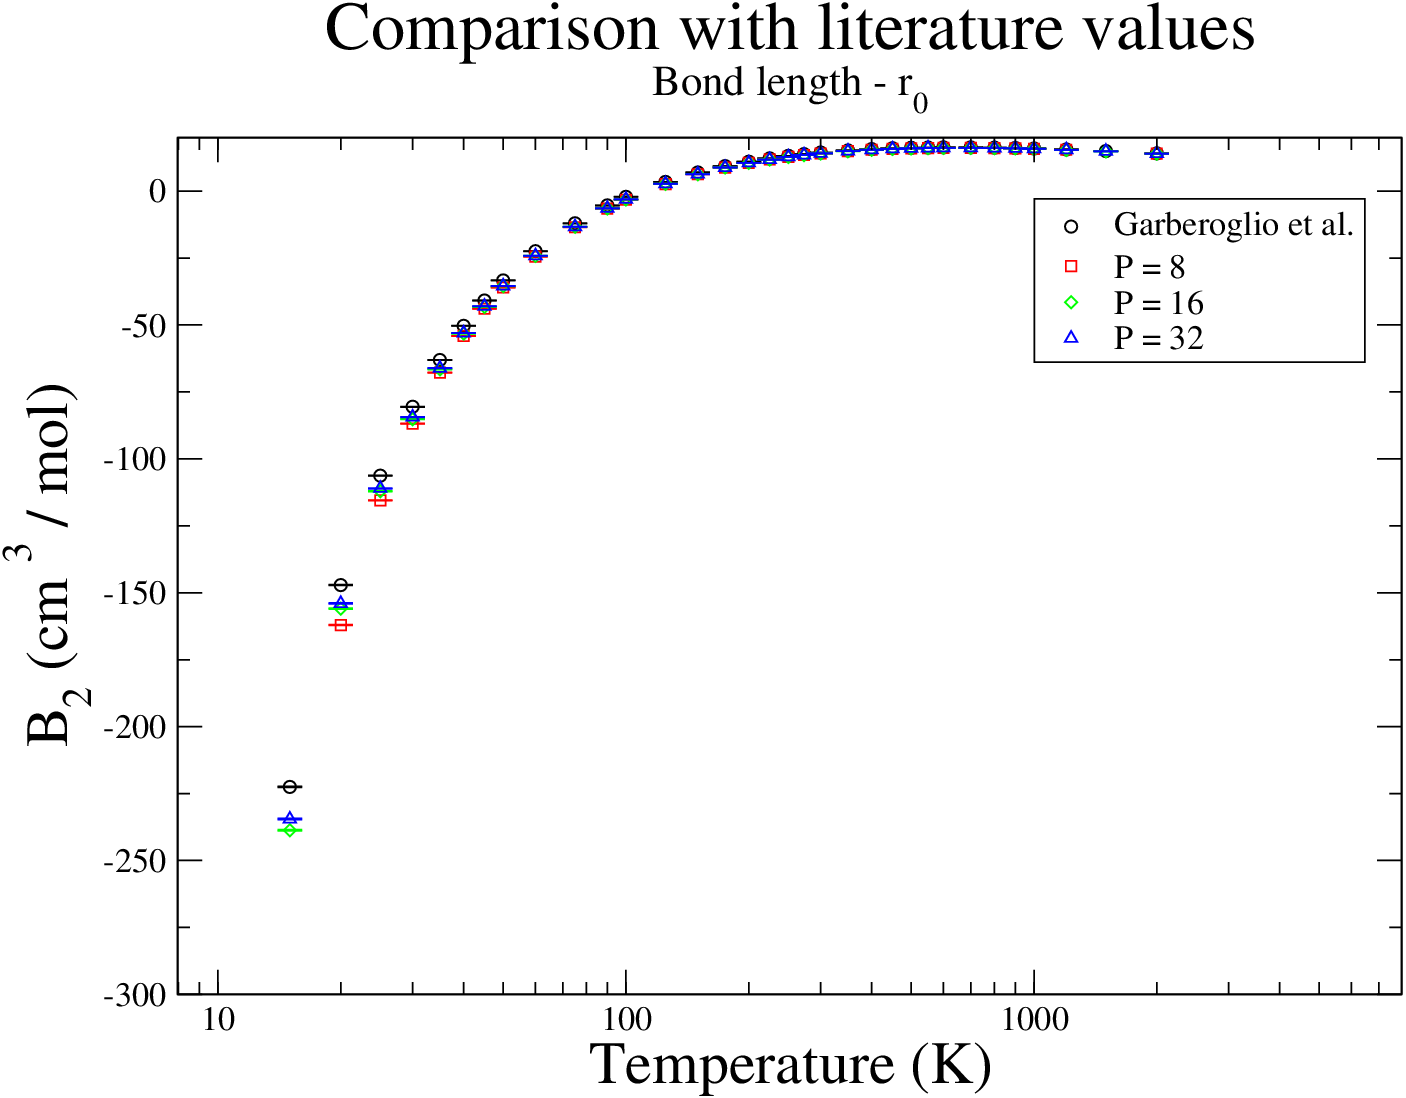
\includegraphics[scale=0.18,keepaspectratio]{8sfGResults.png}
	\end{figure}
	
	\end{frame}

	\begin{frame}
	\frametitle{Bond length \putCitation{Garberoglio2014}- $r_0$}
	\begin{figure}
	\centering
	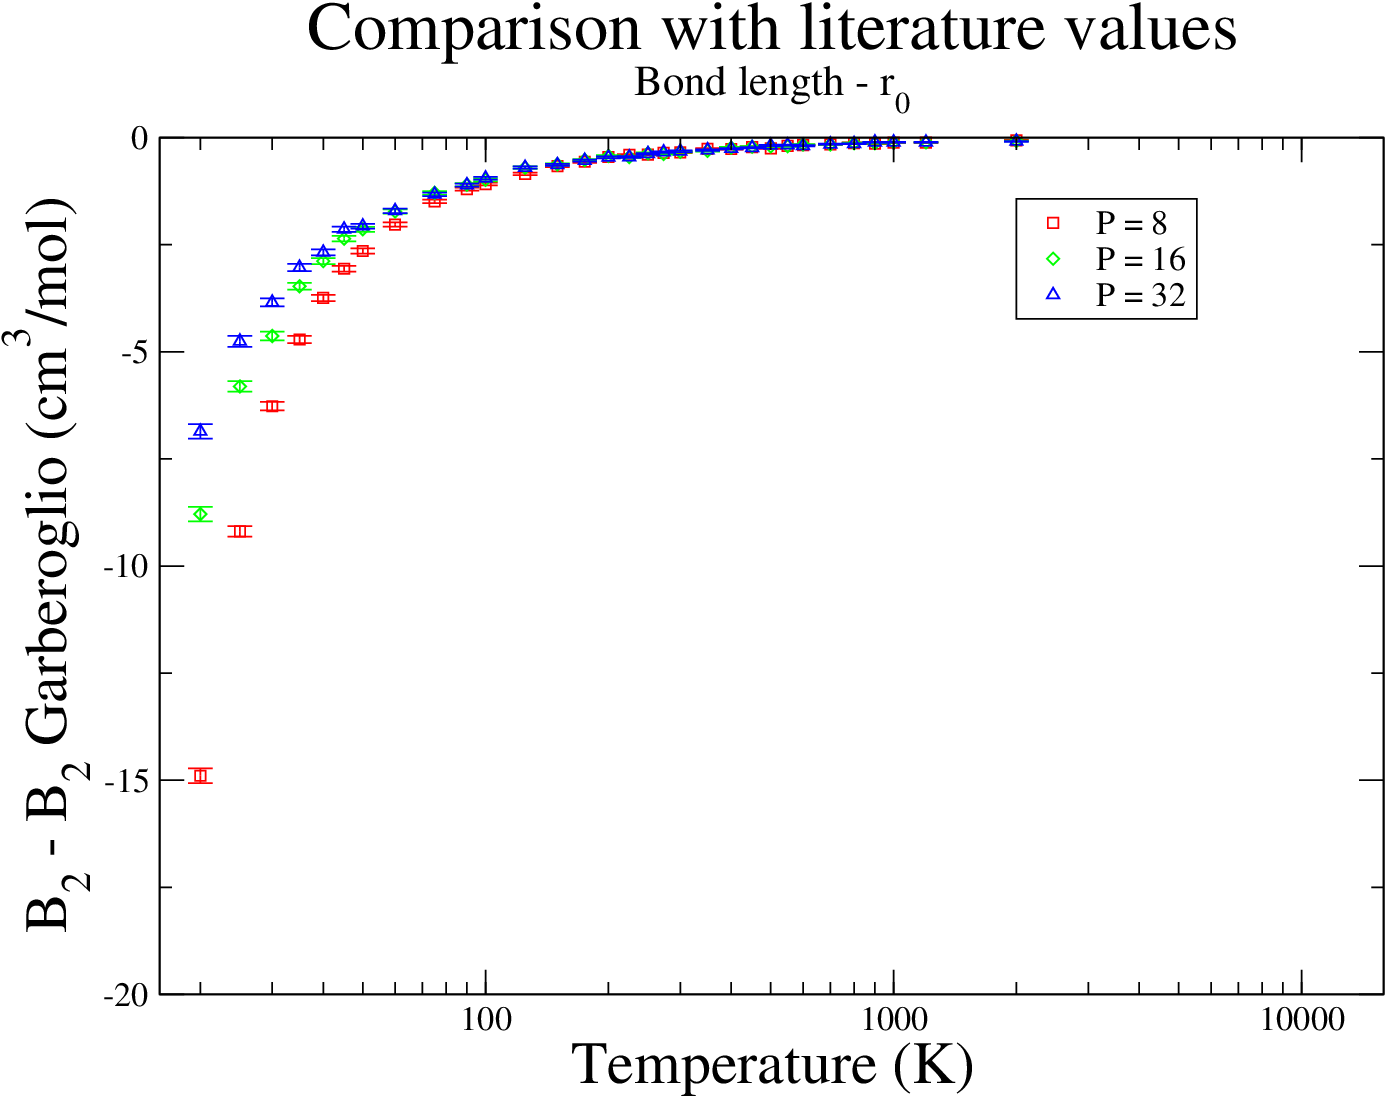
\includegraphics[scale=0.18,keepaspectratio]{8sfGResultsDiff.png}
	\end{figure}
	
	\end{frame}

	\begin{frame}
	\frametitle{Methods to handle flexibility}
	\begin{itemize}
	\justifying
	\item Instead of using ground state bond length ($r_0$) use average bond length at each temperature ($< r >_T$)
	\item Average the bond length values over internal degrees of freedom of each monomer, weighted by the appropriate wave function\putCitation{Garberoglio2012}
	\begin{equation*}
	<r>_T = \displaystyle\sum\limits_{n,J} p(n,J:T) < \chi_{nJ} | r | \chi_{nJ} >
	\end{equation*}
	\noindent where $n$ and $J$ are quantum numbers that define the vibrational and rotational state of $H_2$,respectively, while $\chi_{nJ}$ denotes the corresponding wave-function and \\
	\begin{equation*}
	p(n,J:T) = \frac{(2J + 1) \exp(-E(n,J)/T)}{\displaystyle\sum\limits_{n',J'} (2J' + 1) \exp(-E(n',J')/T)}
	\end{equation*}
	\noindent where $E(n',J')$ is the energy of the $(n',J')$ state
	\end{itemize}
	\end{frame}

	\begin{frame}
	\frametitle{Bond length\putCitation{Garberoglio2014}- $< r >_T$}
	\begin{figure}
	\centering
	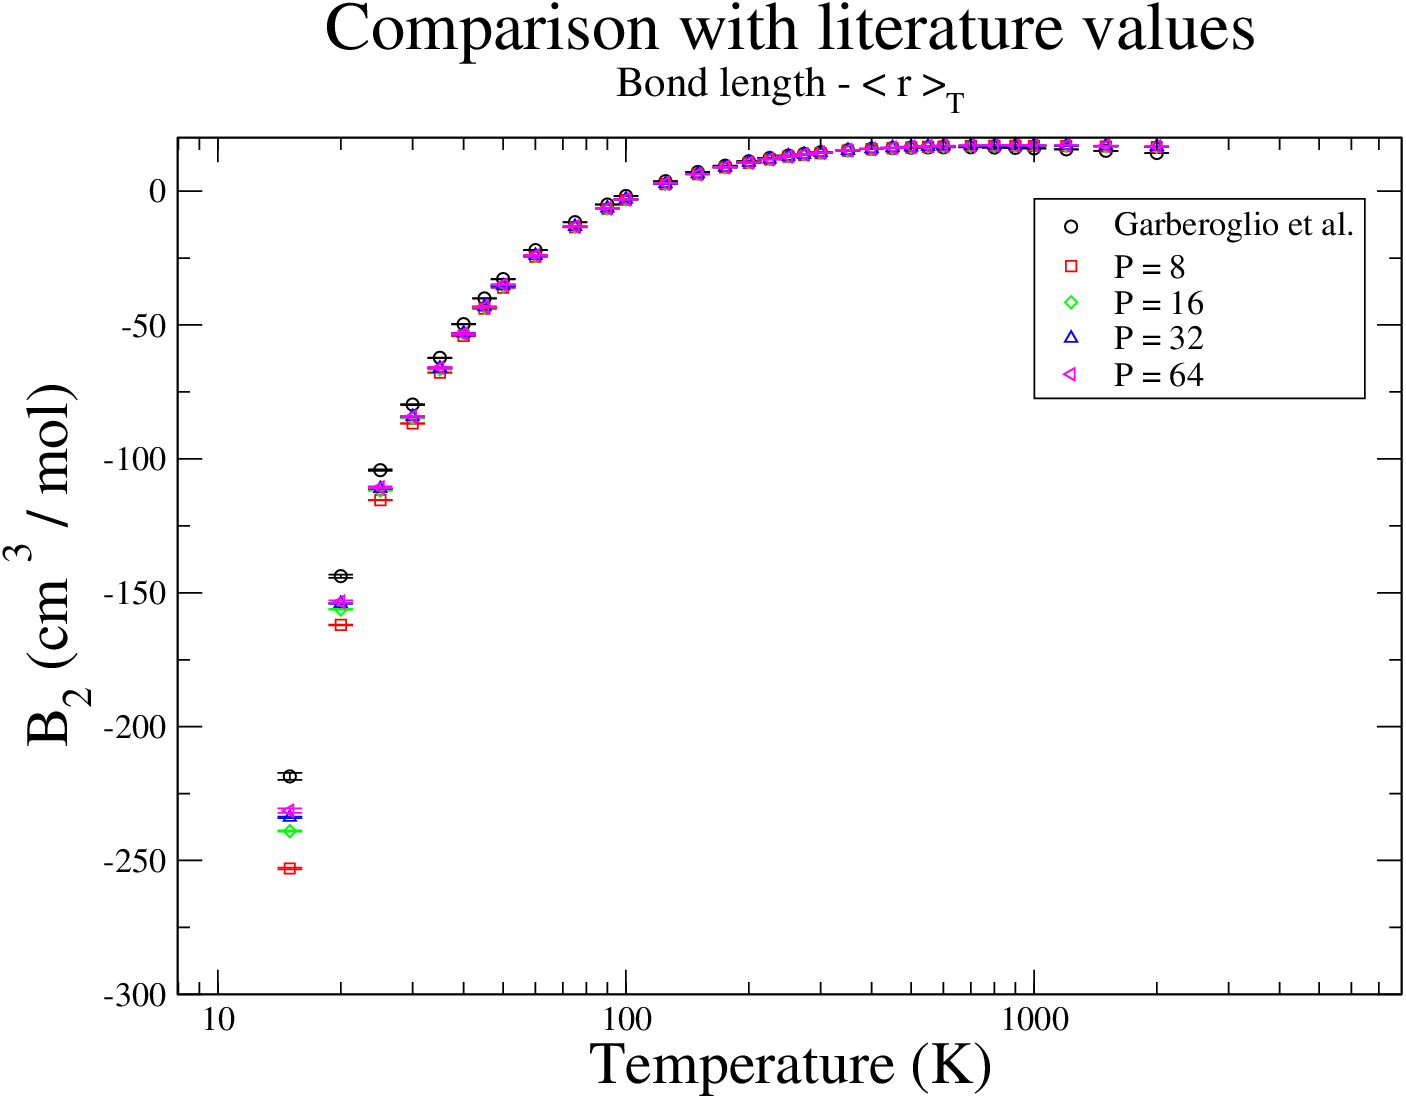
\includegraphics[scale=0.18,keepaspectratio]{8sfTAResults.png}
	\end{figure}
	
	\end{frame}

	\begin{frame}
	\frametitle{Bond length\putCitation{Garberoglio2014} - $< r >_T$}
	\begin{figure}
	\centering
	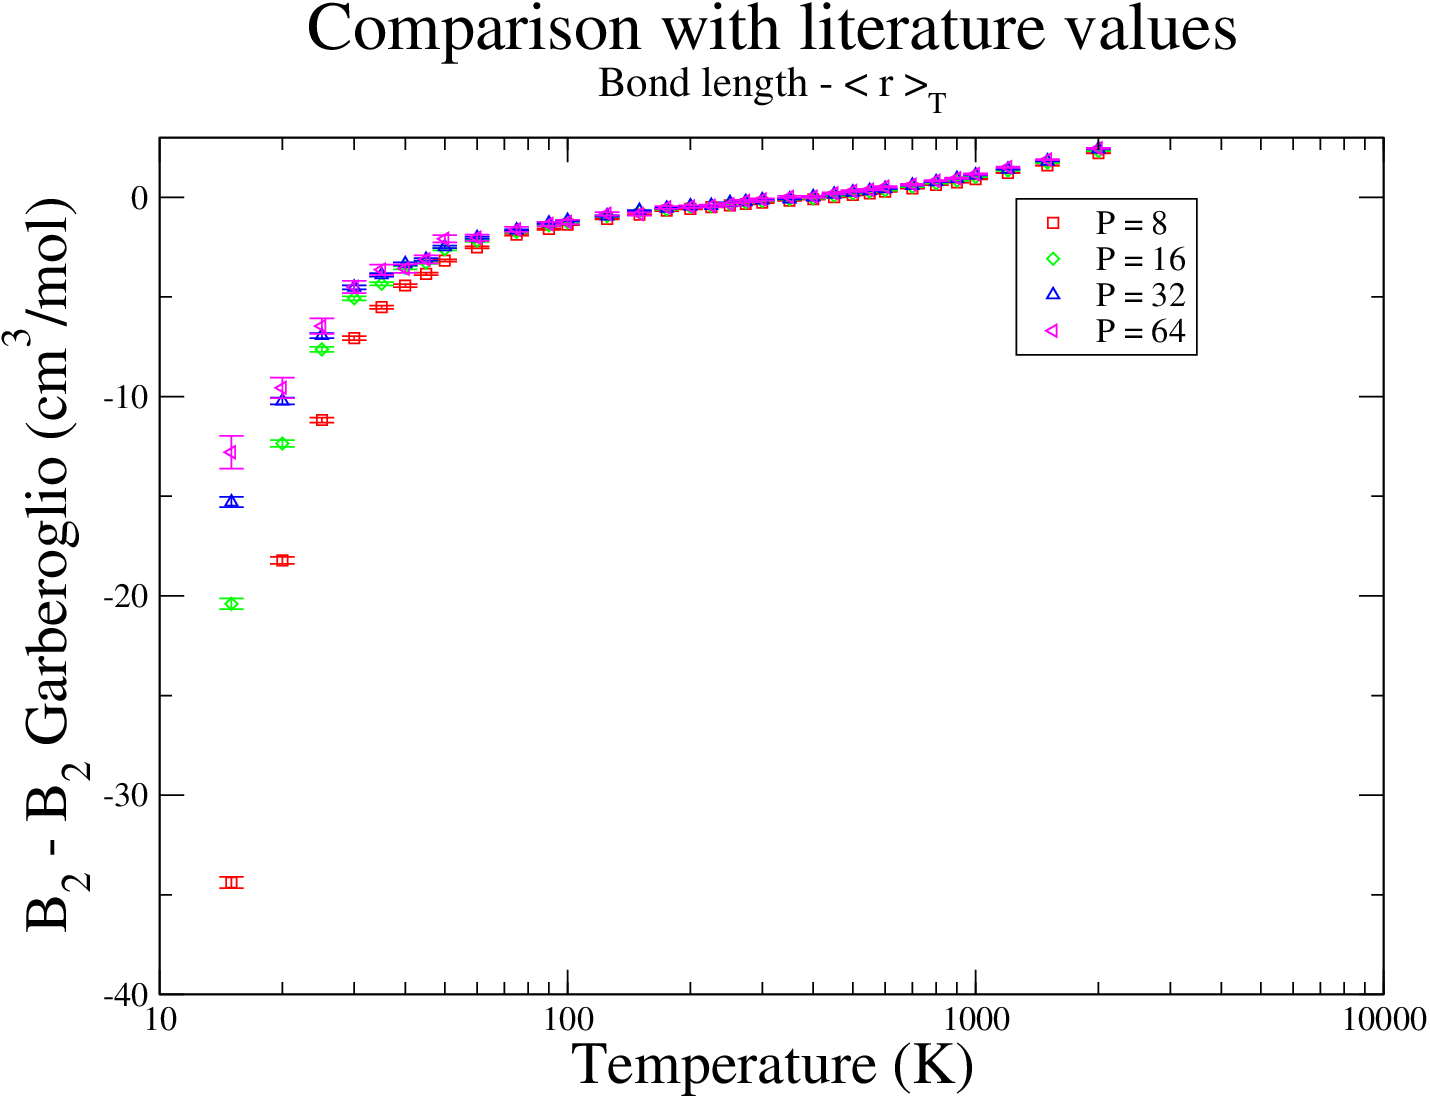
\includegraphics[scale=0.18,keepaspectratio]{8sfTAResultsDiff.png}
	\end{figure}
	
	\end{frame}

	\begin{frame}
	\frametitle{Bond length sampling - Introduction}
	\begin{itemize}
	\justifying
	\item Harmonic energy ($U_h$) of the springs and the intra-molecular potential energy ($U_i$) are the only two factors that affect the probability $\mathcal{P}$ of an image
	\item $U_h$ for adjacent monomers is given by:
	\begin{figure}
	\centering
	\def\svgscale{0.2}
	\input{uHarmonic.pdf_tex}
	\end{figure}
	\begin{equation*}
	\begin{aligned}
	U_h &= \frac{1}{2} \cdot k_h \cdot \displaystyle\sum\limits_{i=0}^P \Big( b_i^2 + b_j^2 - 2 \cdot b_i \cdot b_j \cdot \cos (\theta_{ij}) \Big)\\
	\text{where,} \: j &= i - 1 \: \text{for} \: i \ge 1 , j = P - 1\: \text{for} \: i = 0
	\end{aligned}
	\end{equation*}
	\item Intra-molecular potential that we use in our calculations is from Mielke et al.\putCitation{Mielke2002}
	\end{itemize}
	\end{frame}

	\begin{frame}
	\frametitle{$\mathcal{P}$ - actual probability of a configuration}
	\begin{itemize}
	\justifying
	\item Expression for $\mathcal{P}$ is almost exponential
	\item Consider the argument of the exponential 
	\begin{equation*}
	- \log \mathcal{P} = \displaystyle\sum\limits_{i=0}^P \Bigg\{ k_h \cdot \Big( b_i^2 - b_i \cdot b_j \cdot \cos (\theta_{ij}) \Big) - 2 \cdot \log b_i + \frac{ \beta \cdot U_i (b_i)}{P} \Bigg\}
	\end{equation*}
	\item We can clearly see that it is not quadratic due to the presence of $U_i$
	\item Presence of cross terms such as $b_i \cdot b_j$ makes the bond lengths non-independent of each other
	\end{itemize}
	\end{frame}
	
	\begin{frame}
	\frametitle{Normal mode analysis}
	\begin{columns}[c]
	\begin{column}{6cm}
	\begin{itemize}
	\justifying
	\item Helps choose all bond lengths simultaneously
	\item Consider the combined behavior of all bond lengths as separate modes
	\item Construct matrix with second derivatives of $- \log \mathcal{P}$
	\item Compute eigenvalues $\lambda_i$ and eigenvectors $\vec{A_i}$ to separate out independent modes
	\item Evaluate new bond lengths simultaneously 
	\end{itemize}
	\end{column}

	\begin{column}{4cm}
	\begin{figure}
	\centering
	\def\svgscale{0.3}
	\input{differentModes.pdf_tex}
	\end{figure}
	\end{column}
	\end{columns}
	\end{frame}

	\begin{frame}
	\frametitle{Bond length\putCitation{Garberoglio2014} - flexible}
	\begin{figure}
	\centering
	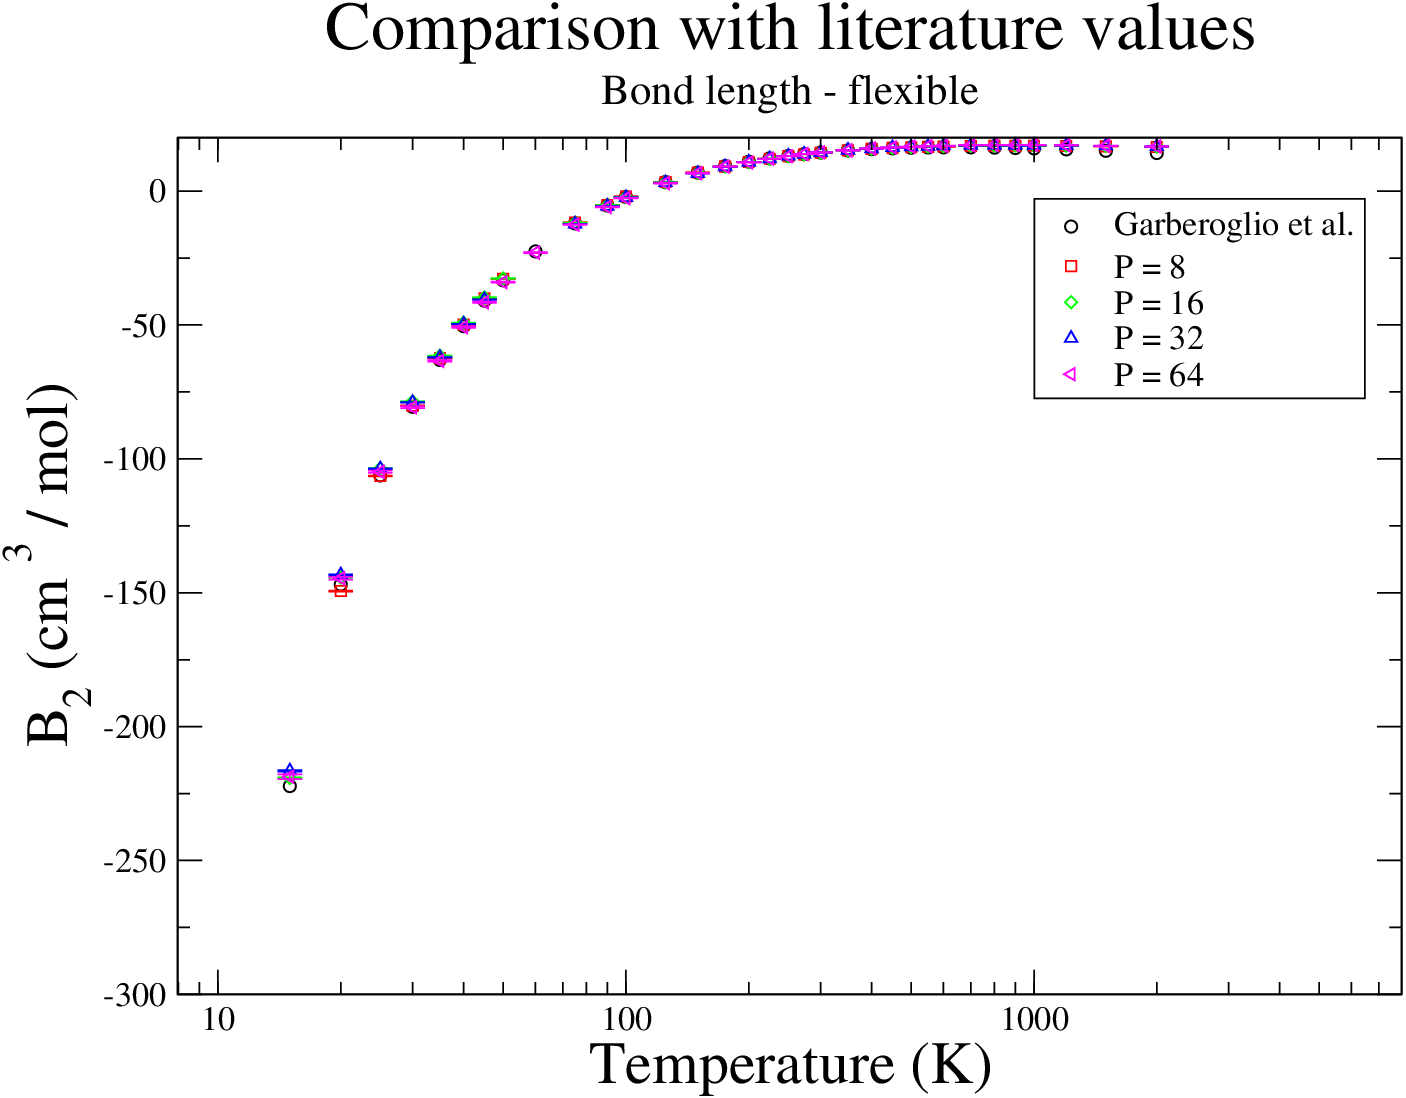
\includegraphics[scale=0.18,keepaspectratio]{8svBLResults.png}
	\end{figure}
	
	\end{frame}

	\begin{frame}
	\frametitle{Bond length\putCitation{Garberoglio2014} - flexible}
	\begin{figure}
	\centering
	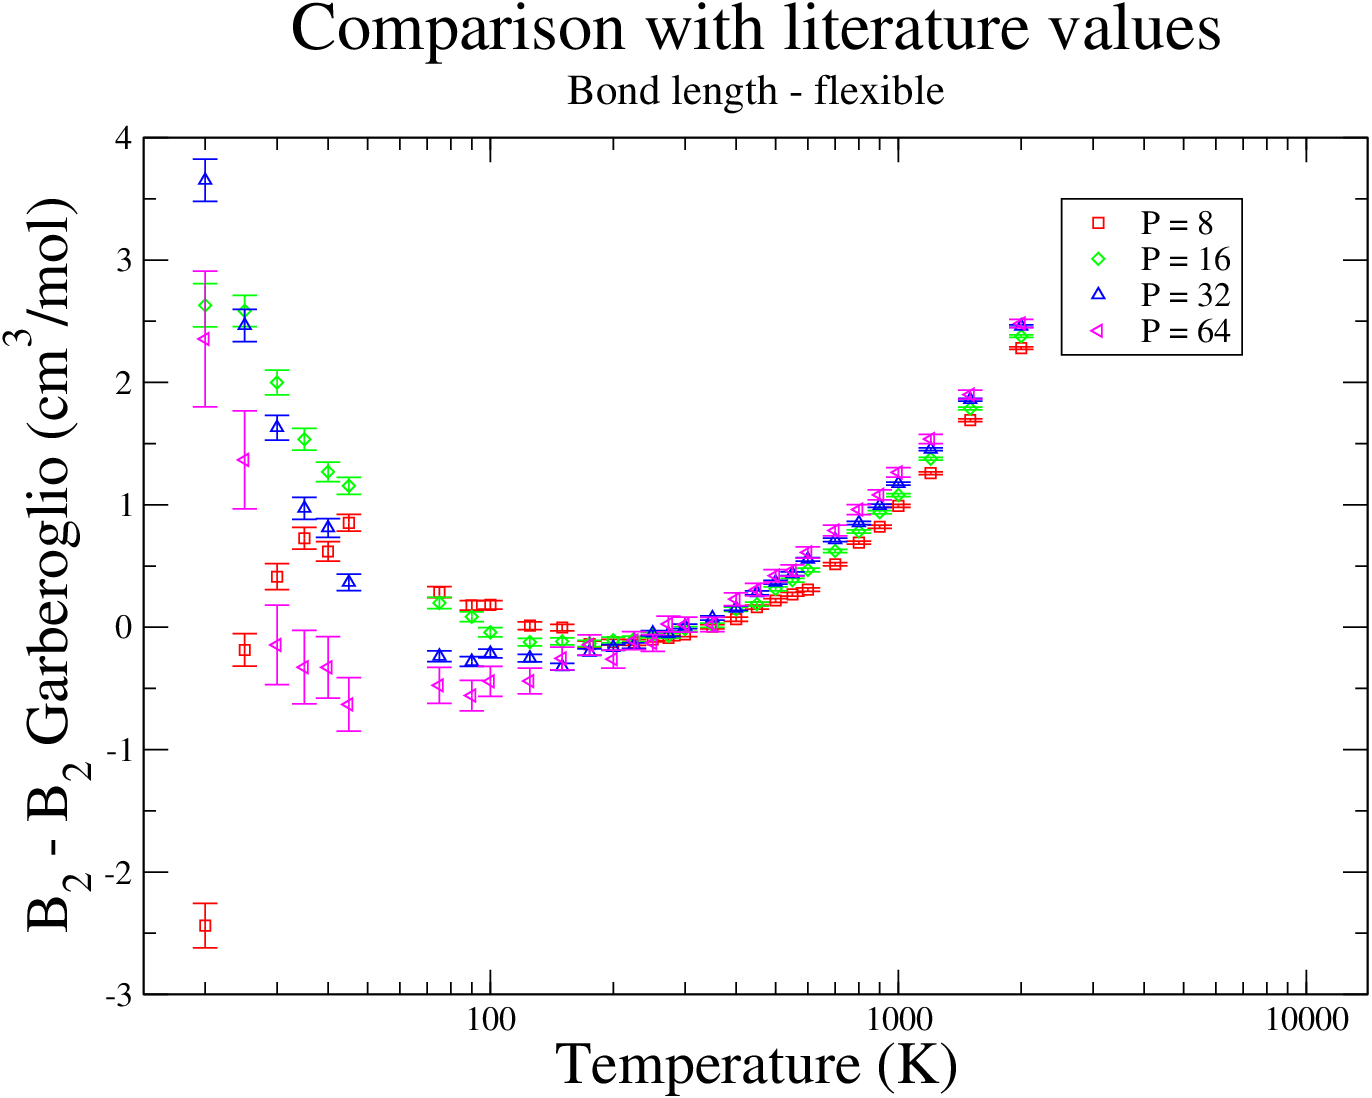
\includegraphics[scale=0.18,keepaspectratio]{8svBLResultsDiff.png}
	\end{figure}
	\end{frame}

	\begin{frame}
	\frametitle{Summary and future work}
	\begin{itemize}
	\justifying
	\item We have developed a bond length sampling algorithm that can be used to compute virial coefficients for flexible diatomic molecules
	\item We applied the algorithm for $H_2$ molecule and the resulting second virial coefficients are not in perfect agreement with literature data      
	\item Fix remaining issues and improve efficiency of the move
	\item Apply the algorithm for other diatomic systems like $N_2$
	\item Extend the algorithm to other complicated systems like water
	\end{itemize}
	\end{frame}
	
	\begin{frame}
	\setbeamertemplate{headline}{}
	\frametitle{Acknowledgment}
	\begin{itemize}
	\item My advisor Dr. David Kofke
	\item Dr. Andrew Schultz
	\item Members of the Kofke group
	\item Funding:
	\begin{figure}
	\centering
	
\includegraphics[width=5cm,keepaspectratio]{nsfLogo.png}
	\end{figure}
	\item Computational resources:
	\begin{figure}
	
\includegraphics[width=5cm,keepaspectratio]{ccrLogo.jpg}
	\end{figure}
	\item We would like to thank Dr. Allan H. Harvey for insightful discussions
	\end {itemize}
	\end{frame}

	\begin{frame}
	\frametitle{Thank you for your attention!}
	\begin{center}
	\huge{Questions???}
	\end{center}
	\end{frame}

	\begin{frame}
	\frametitle{$P_{act}$}
	\begin{itemize}
	\item Let $P_{act} = \exp (-z_{act})$ where $z_{act}$ can be defined as follows:-
	\begin{equation*} \label {zact}
	z_{act} = \displaystyle\sum\limits_{i=0}^P \Bigg\{ k_h \cdot \Big( b_i^2 - b_i \cdot b_j \cdot \cos (\theta_{ij}) \Big) - 2 \cdot \log b_i + \frac{ \beta \cdot U_i (b_i)}{P} \Bigg\}
	\end{equation*}
	\item Since $z_{act}$ is not quadratic, it is not easy to sample from
	\item All bond lengths not independent of each other
	\end{itemize}
	\end{frame}

	\begin{frame}
	\frametitle{Assumptions and modifications}
	\begin{itemize}
	\justifying
	\item $z_{act}$ is given by:
	\begin{equation*}
	z_{act} = \displaystyle\sum\limits_{i=0}^P \Bigg\{ k_h \cdot \Big( b_i^2 - b_i \cdot b_j \cdot \cos (\theta_{ij}) \Big) - 2 \cdot \log b_i + \frac{ \beta \cdot U_i (b_i)}{P} \Bigg\}
	\end{equation*}
	\item Finding $b_{min}$, given as the solution of $\frac{\partial z_{act}}{\partial b_i} \Big|_{b_i = b_{min}} = 0$, before each move can be very inefficient
	\item Let $z_{act}^*$ be given by:
	\begin{equation*}
	z_{act}^* = \displaystyle\sum\limits_{i=0}^P \Bigg\{ k_h \cdot \Big( b_i^2 - b_i \cdot b_j \Big) - \frac{2 \cdot \log b_i}{P} + \frac{ \beta \cdot U_i (b_i)}{P} \Bigg\}
	\end{equation*}
	\item Find $b_{min}$ using $\frac{\partial z_{act}^*}{\partial b_i} \Big|_{b_i = b_{min}} = 0$, set $\displaystyle\frac{\partial z_{act}}{\partial b_i} = \displaystyle\frac{\partial z_{act}^*}{\partial b_i}$ and solve for $\theta_{ij}$
	\end{itemize}
	\end{frame}

	\begin{frame}
	\frametitle{Assumptions and modifications}
	\begin{itemize}
	\item Let $\frac{\partial z_{act}}{\partial b_i} = \frac{\partial z_{act}^*}{\partial b_i}$ solve for $\cos (\theta_{ij})$
	\item $\cos (\theta_{ij}) = 1 - \frac{P-1}{P \cdot k_h \cdot b_i^2}$
	\item Compute $b_{min}$ using $\frac{\partial z_{act}}{\partial b_i} \Bigg|_{b_i = b_{min}} = \frac{\partial z_{act}^*}{\partial b_i} \Bigg|_{b_i = b_{min}} = 0$
	\end{itemize}
	\end{frame}

	\begin{frame}
	\frametitle{Conclusions}
	\begin{itemize}
	\item Let $\frac{\partial z_{act}}{\partial b_i} = \frac{\partial z_{act}^*}{\partial b_i}$ solve for $\cos (\theta_{ij})$
	\item $\cos (\theta_{ij}) = 1 - \frac{P-1}{P \cdot k_h \cdot b_i^2}$
	\item Compute $b_{min}$ using $\frac{\partial z_{act}}{\partial b_i} \Bigg|_{b_i = b_{min}} = \frac{\partial z_{act}^*}{\partial b_i} \Bigg|_{b_i = b_{min}} = 0$
	\end{itemize}
	\end{frame}

	\begin{frame}
	\frametitle{Future work}
	\begin{itemize}
	\item Let $\frac{\partial z_{act}}{\partial b_i} = \frac{\partial z_{act}^*}{\partial b_i}$ solve for $\cos (\theta_{ij})$
	\item $\cos (\theta_{ij}) = 1 - \frac{P-1}{P \cdot k_h \cdot b_i^2}$
	\item Compute $b_{min}$ using $\frac{\partial z_{act}}{\partial b_i} \Bigg|_{b_i = b_{min}} = \frac{\partial z_{act}^*}{\partial b_i} \Bigg|_{b_i = b_{min}} = 0$
	\end{itemize}
	\end{frame}

	\begin{frame}
	\frametitle{Future work}
	\begin{itemize}
	\item Let $\frac{\partial z_{act}}{\partial b_i} = \frac{\partial z_{act}^*}{\partial b_i}$ solve for $\cos (\theta_{ij})$
	\item $\cos (\theta_{ij}) = 1 - \frac{P-1}{P \cdot k_h \cdot b_i^2}$
	\item Compute $b_{min}$ using $\frac{\partial z_{act}}{\partial b_i} \Bigg|_{b_i = b_{min}} = \frac{\partial z_{act}^*}{\partial b_i} \Bigg|_{b_i = b_{min}} = 0$
	\end{itemize}
	\end{frame}
	
\end{document}
